
\chapter{Patchwork}

\section{Zeitpläne}

\begin{figure}[!ht]
    \centering
    \begin{minipage}{.48\textwidth}
        \centering
        \begin{tikzpicture}
            \node [inner sep=0pt,,outer sep=0pt,clip,rounded corners=0.15cm] (image) at (0,0) {\includegraphics[width=0.75\linewidth]{res/pictures/assets/time-board-side-1.png}};
            \drawshadow{image}
        \end{tikzpicture}
    \end{minipage}
    \hfill
    \begin{minipage}{.48\textwidth}
        \centering
        \begin{tikzpicture}
            \node [inner sep=0pt,,outer sep=0pt,clip,rounded corners=0.15cm] (image) at (0,0) {\includegraphics[width=0.75\linewidth]{res/pictures/assets/time-board-side-2.png}};
            \drawshadow{image}
        \end{tikzpicture}
    \end{minipage}
    \vspace*{-0.05cm}
    \caption{Die zwei Seiten des Zeitplans}
    \label{fig:patchwork-time-board}
\end{figure}

\section{Ablagepläne}

\begin{figure}[!ht]
    \centering
    \begin{minipage}{.48\textwidth}
        \centering
        \begin{tikzpicture}
            \node [inner sep=0pt,,outer sep=0pt,clip,rounded corners=0.15cm] (image) at (0,0) {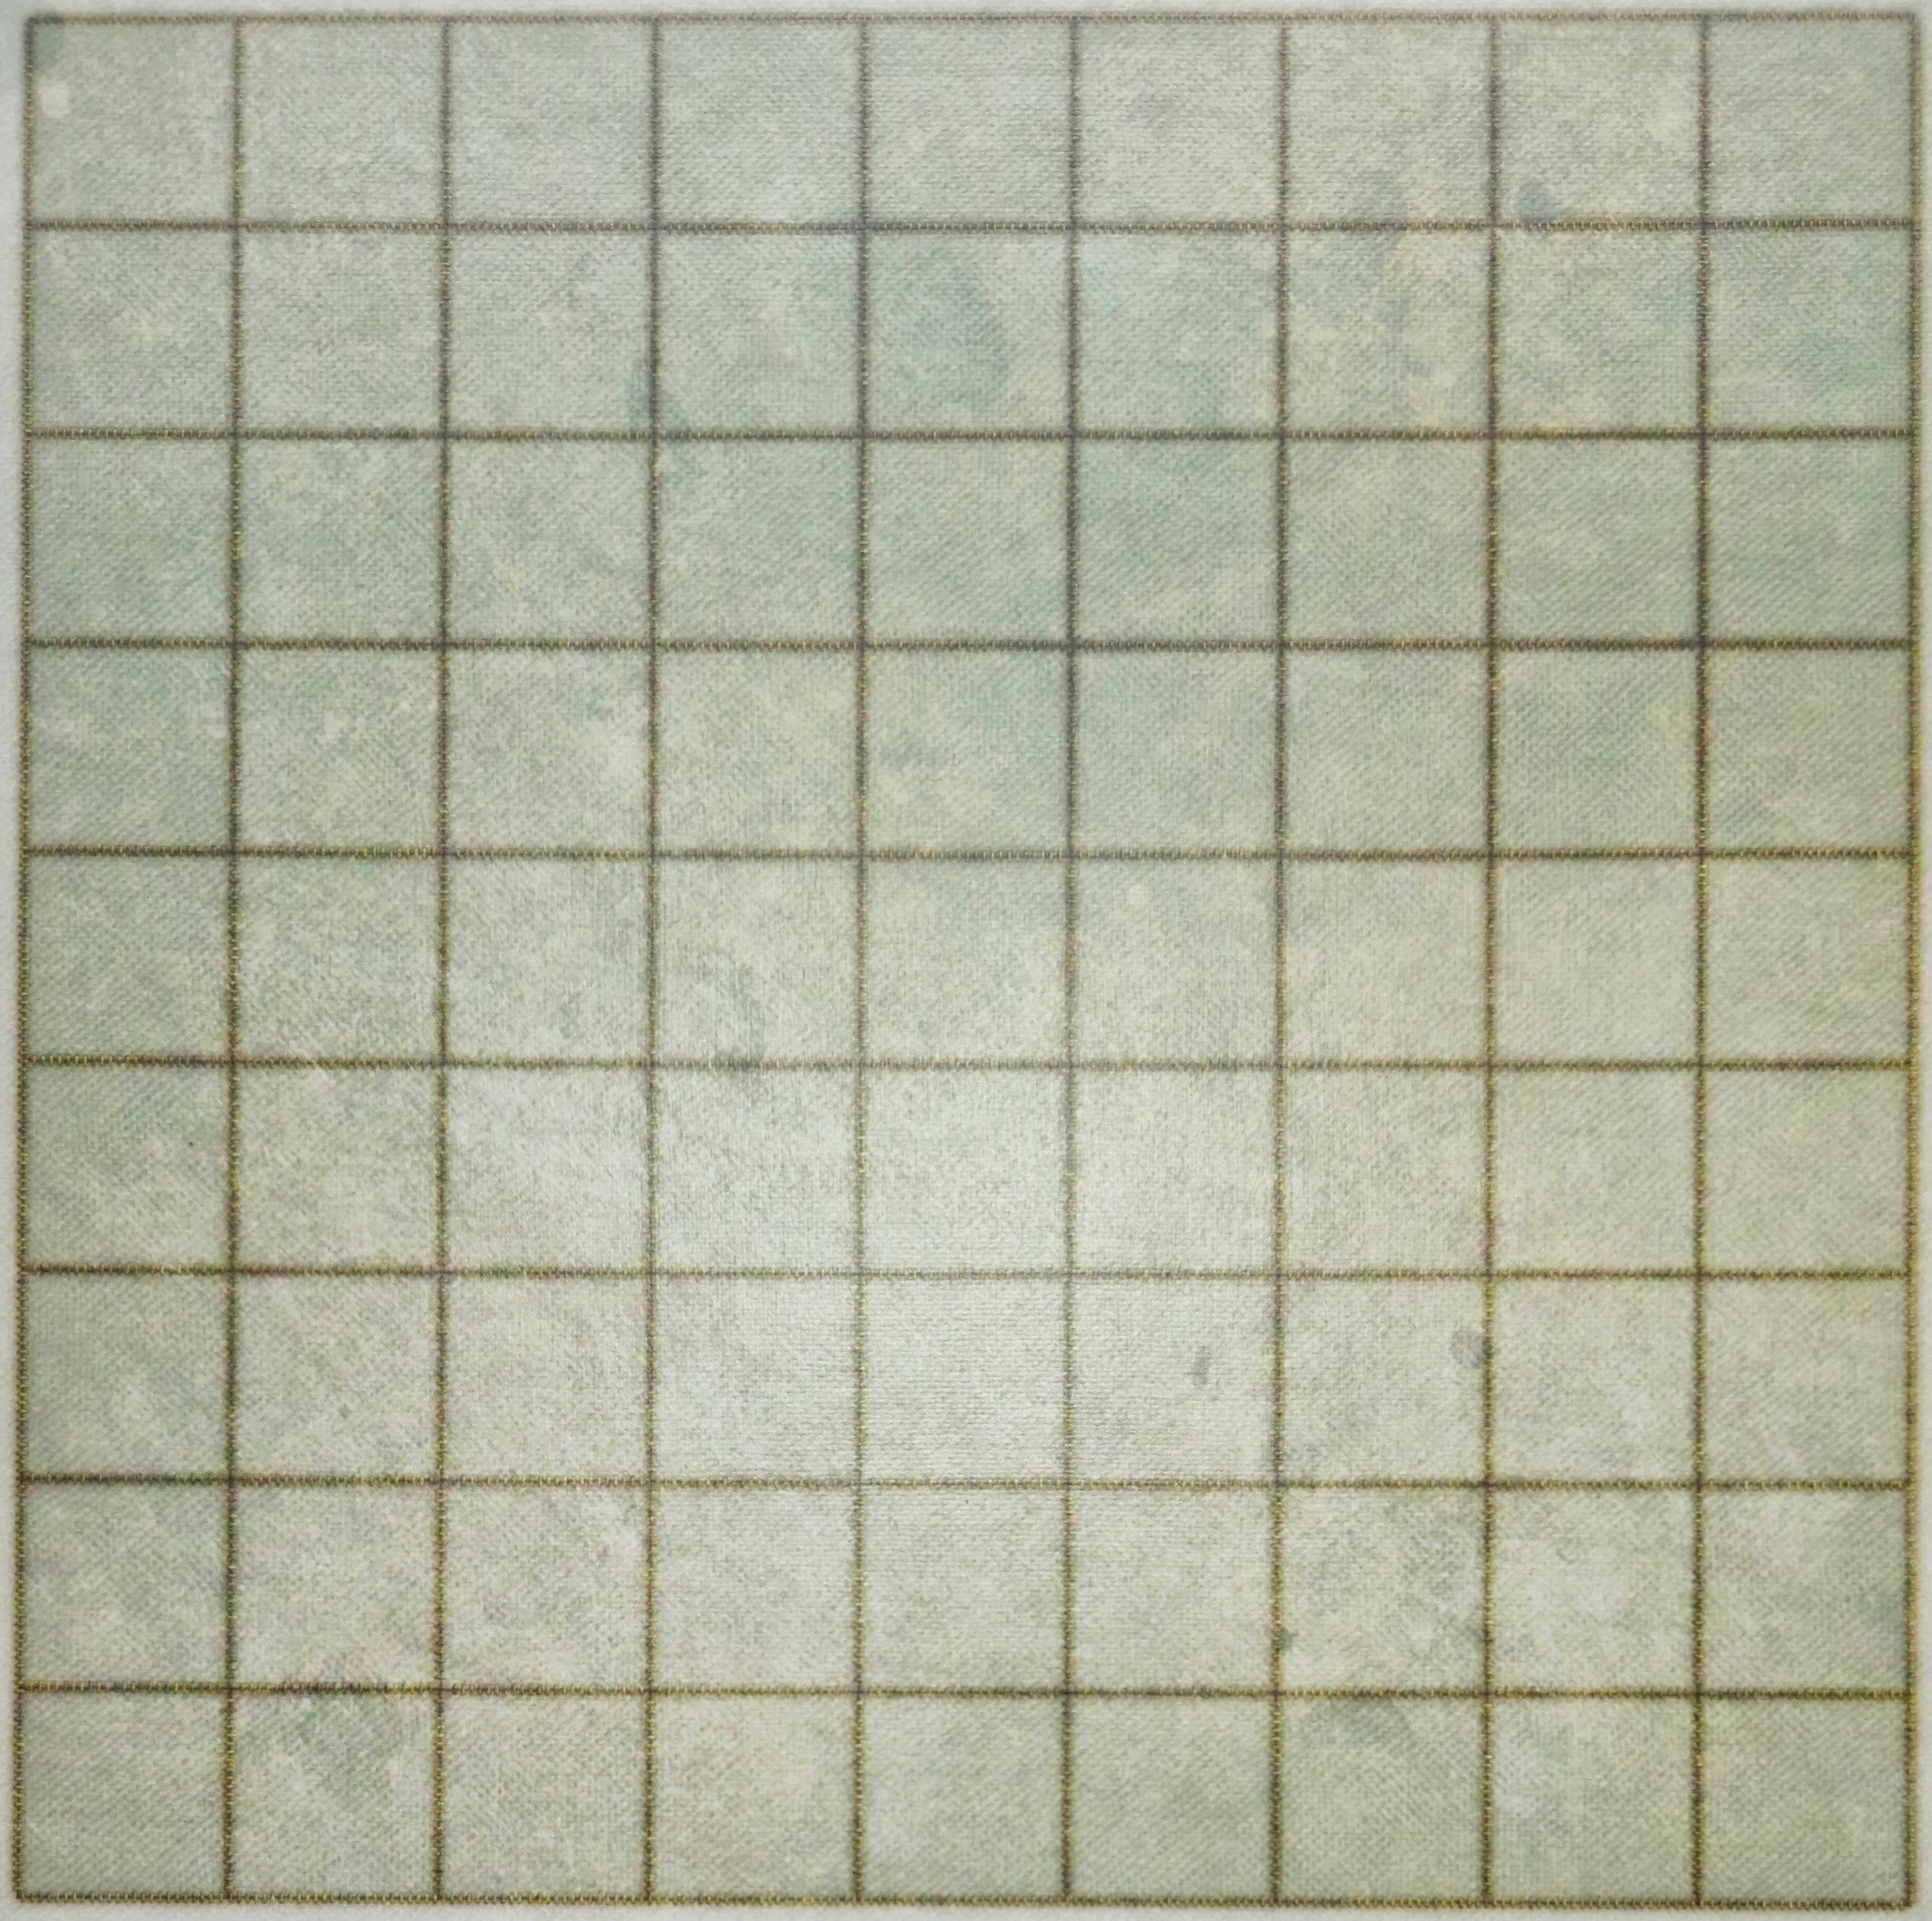
\includegraphics[width=0.75\linewidth]{res/pictures/assets/board-player-1.png}};
            \drawshadow{image}
        \end{tikzpicture}
    \end{minipage}
    \hfill
    \begin{minipage}{.48\textwidth}
        \centering
        \begin{tikzpicture}
            \node [inner sep=0pt,,outer sep=0pt,clip,rounded corners=0.15cm] (image) at (0,0) {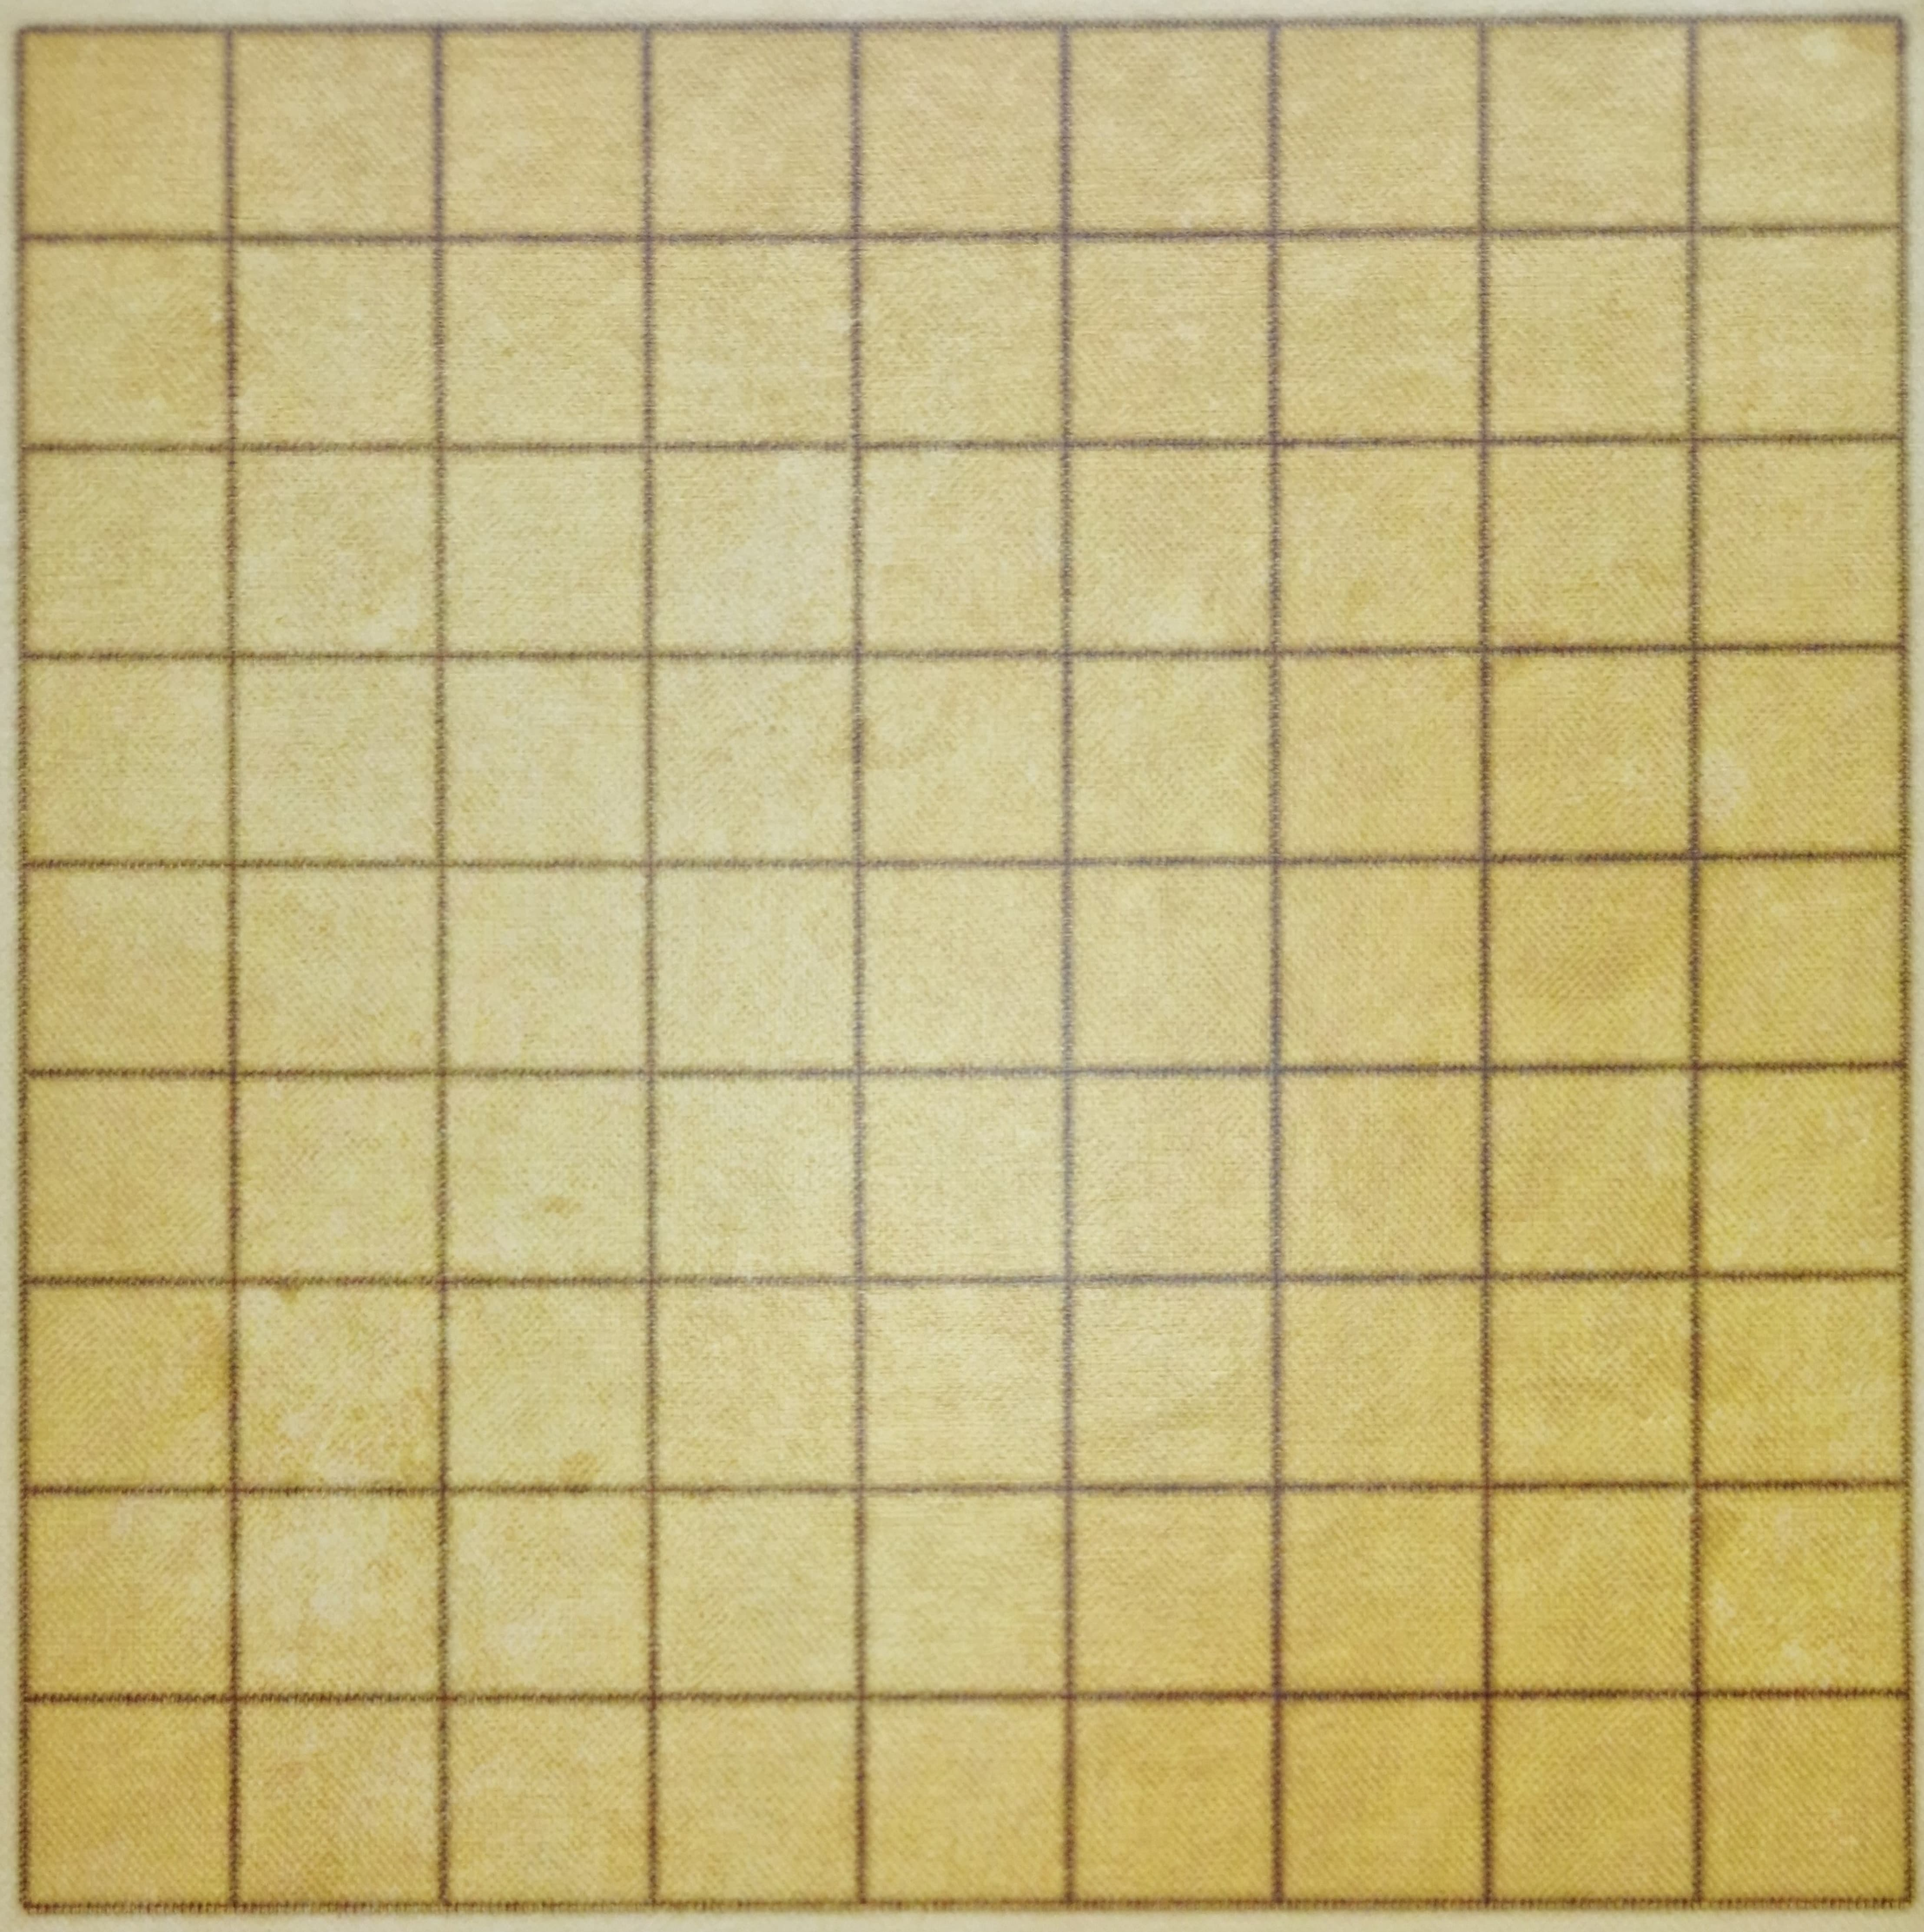
\includegraphics[width=0.75\linewidth]{res/pictures/assets/board-player-2.png}};
            \drawshadow{image}
        \end{tikzpicture}
    \end{minipage}
    \vspace*{-0.05cm}
    \caption[Ablagepläne der Spieler]{Ablagepläne (Decken) der Spieler}
    \label{fig:patchwork-player-quilt-board}
\end{figure}

\pagebreak

\section{Flicken}
\label{anhang:section-patchwork-patches}

% \setlength{\tabcolsep}{5pt}

\begin{longtable}[t]{|c|c|c|c|c|c|c|}
    \hline
    \raisebox{0pt}[3ex][2ex]{Flicken}                                                                                                                 & ID   & Felder & \makecell{ Knopf                                              \\ Kosten } & \makecell{ Zeit \\ Kosten } & \makecell{ Knopf \\ Einkommen } & $\frac{\text{Knopfeinkommen}}{\text{Felder}\, \cdot\, \text{Zeitkosten}}$ \\ \hline
    \endfirsthead
    \multicolumn{7}{c}{\tablename\ \thetable\ -- \textit{Fortsetzung von der vorherigen Seite}}                                                                                                                                       \\
    \hline
    \raisebox{0pt}[3ex][2ex]{Flicken}                                                                                                                 & ID   & Felder & \makecell{ Knopf                                              \\ Kosten } & \makecell{ Zeit \\ Kosten } & \makecell{ Knopf \\ Einkommen } & $\frac{\text{Knopfeinkommen}}{\text{Felder}\, \cdot\, \text{Zeitkosten}}$ \\ \hline
    \endhead
    \hline \multicolumn{7}{r}{\textit{Fortsetzung auf der nächsten Seite}}                                                                                                                                                            \\
    \endfoot
    \hline
    \caption{Alle 33 Flicken in Patchwork}
    \label{tabelle:patchwork-patches}
    \endlastfoot
    \adjustbox{valign=m, max width=0.2\textwidth, max height=0.1\textheight}{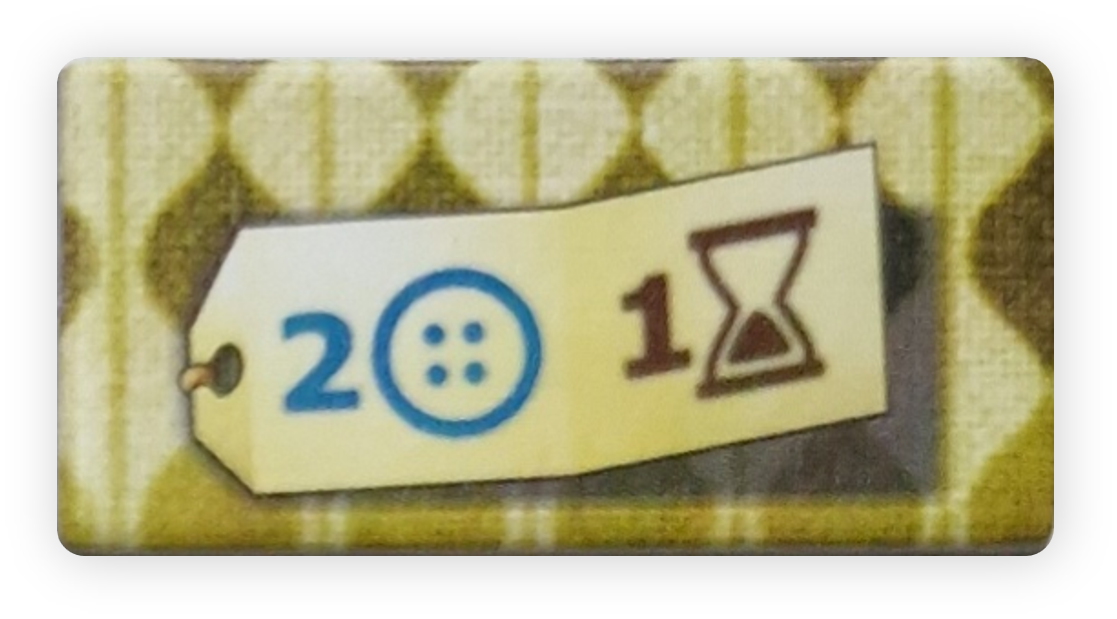
\includegraphics[width=0.2\textwidth]{res/pictures/assets/00-front.png}} & $0$  & $2$    & $2$              & $1$ & $0$ & $0$                            \\ \hline
    \adjustbox{valign=m, max width=0.2\textwidth, max height=0.1\textheight}{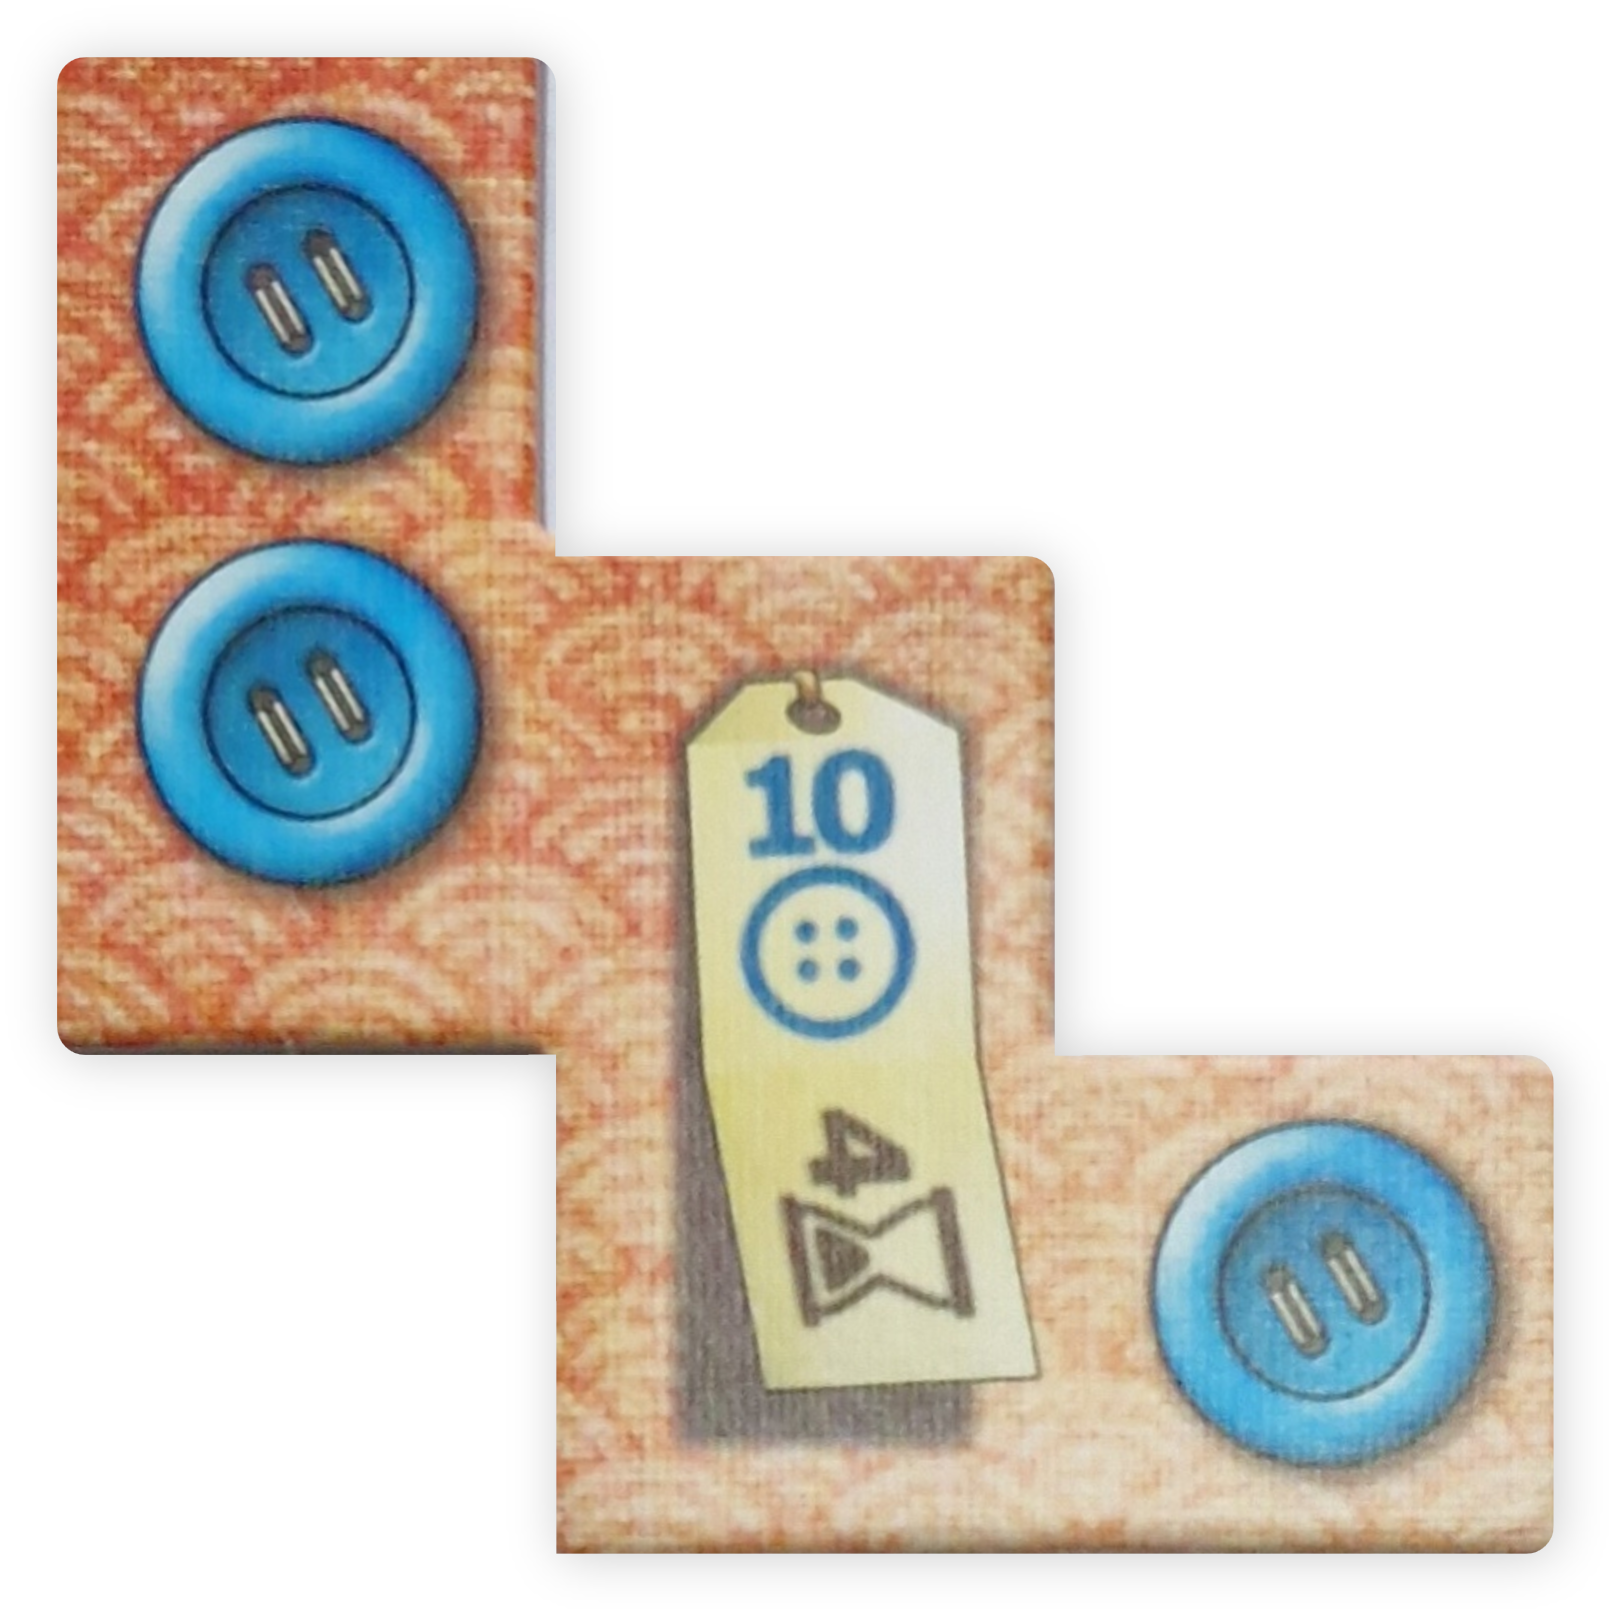
\includegraphics[width=0.2\textwidth]{res/pictures/assets/01-front.png}} & $1$  & $5$    & $10$             & $4$ & $3$ & $\frac{3}{20} = 0{,}15$        \\ \hline
    \adjustbox{valign=m, max width=0.2\textwidth, max height=0.1\textheight}{\includegraphics[width=0.2\textwidth]{res/pictures/assets/02-front.png}} & $2$  & $8$    & $5$              & $3$ & $1$ & $\frac{1}{24} \approx 0{,}042$ \\ \hline
    \adjustbox{valign=m, max width=0.2\textwidth, max height=0.1\textheight}{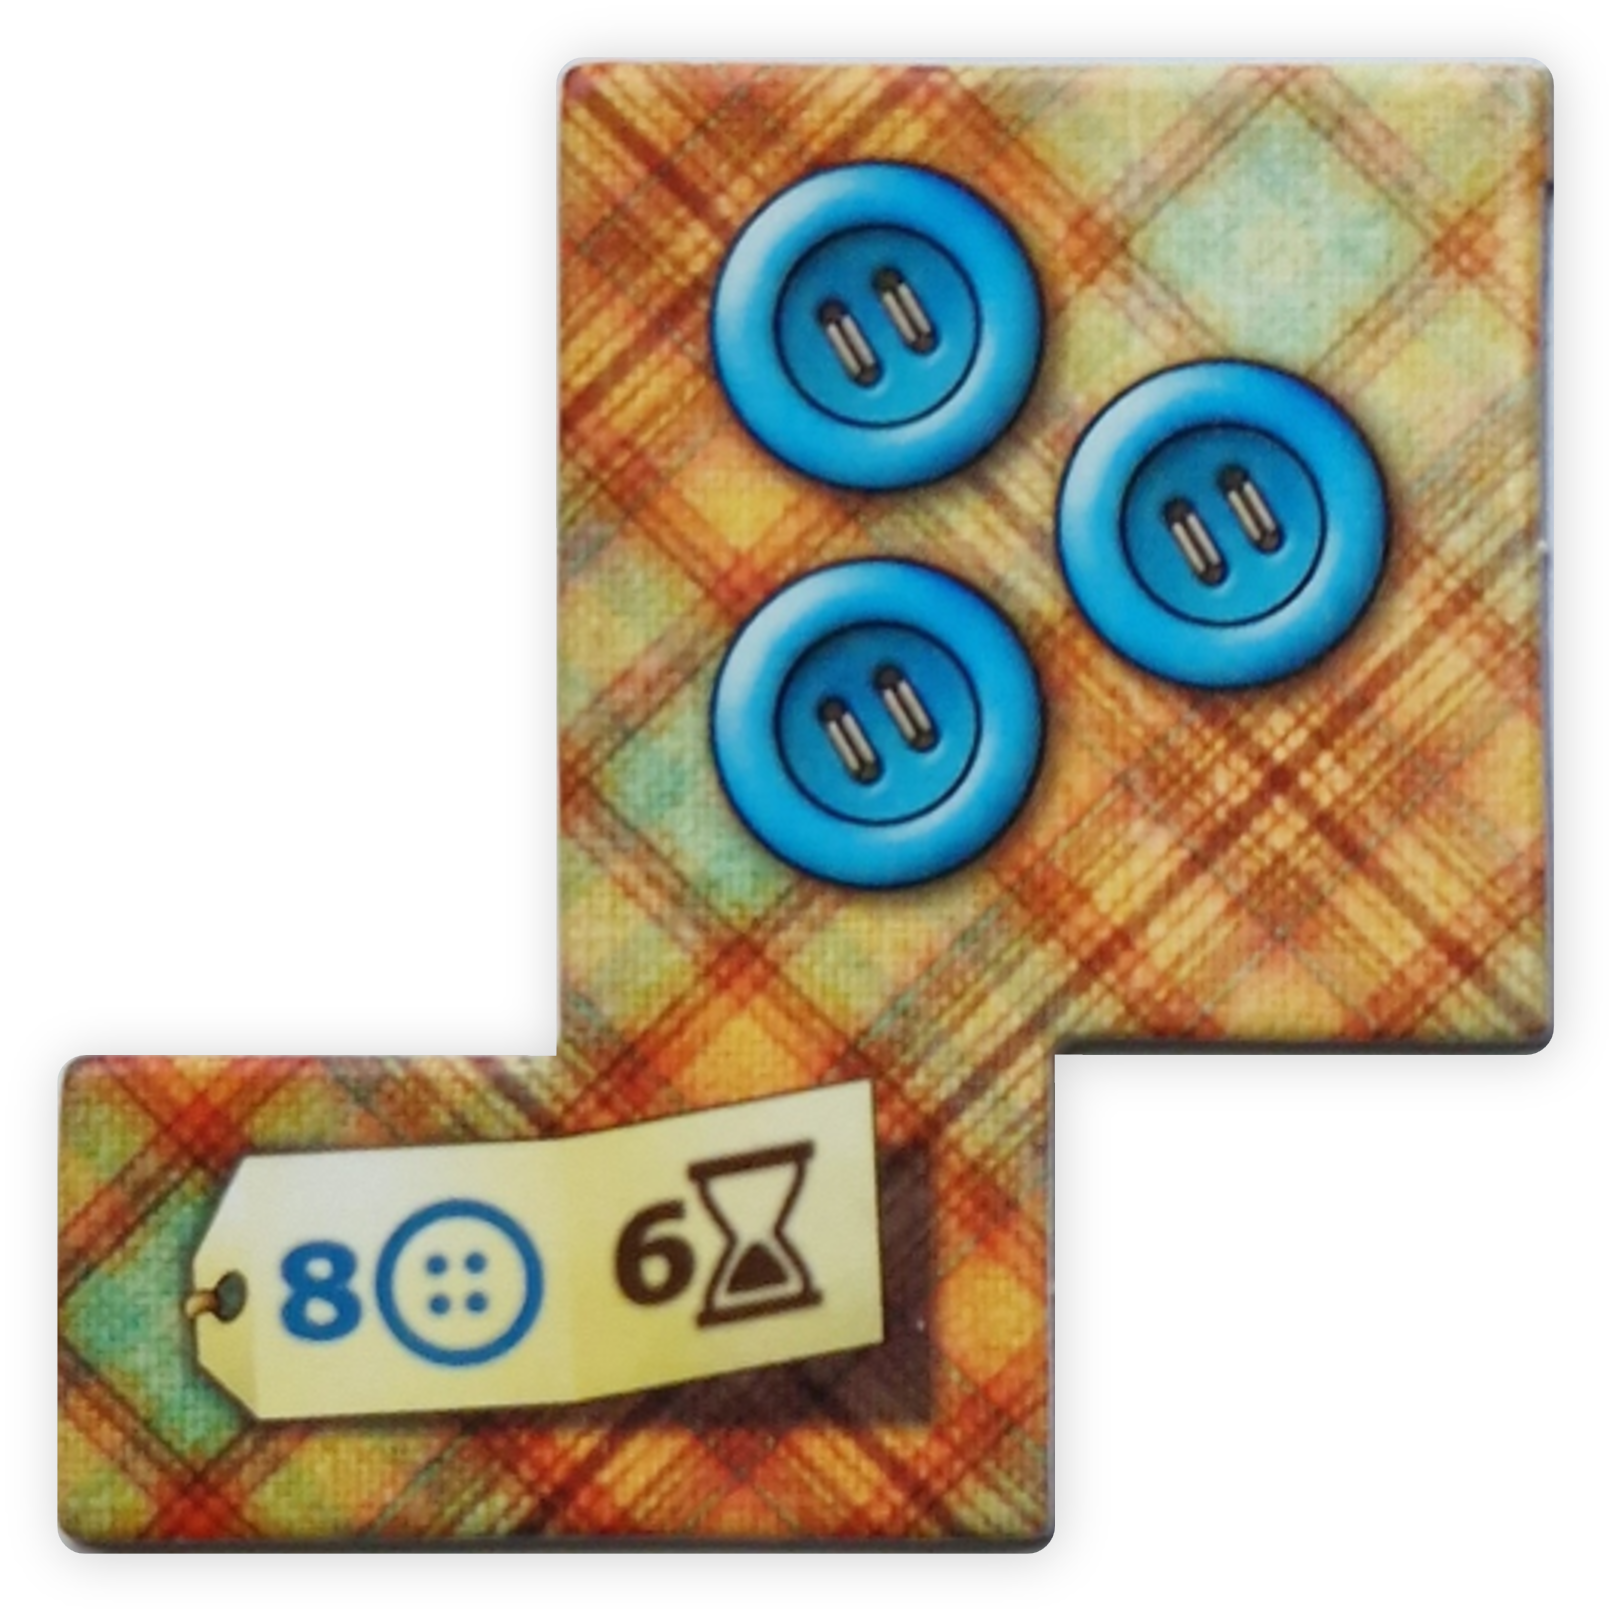
\includegraphics[width=0.2\textwidth]{res/pictures/assets/03-front.png}} & $3$  & $6$    & $8$              & $6$ & $3$ & $\frac{1}{12} \approx 0{,}083$ \\ \hline
    \adjustbox{valign=m, max width=0.2\textwidth, max height=0.1\textheight}{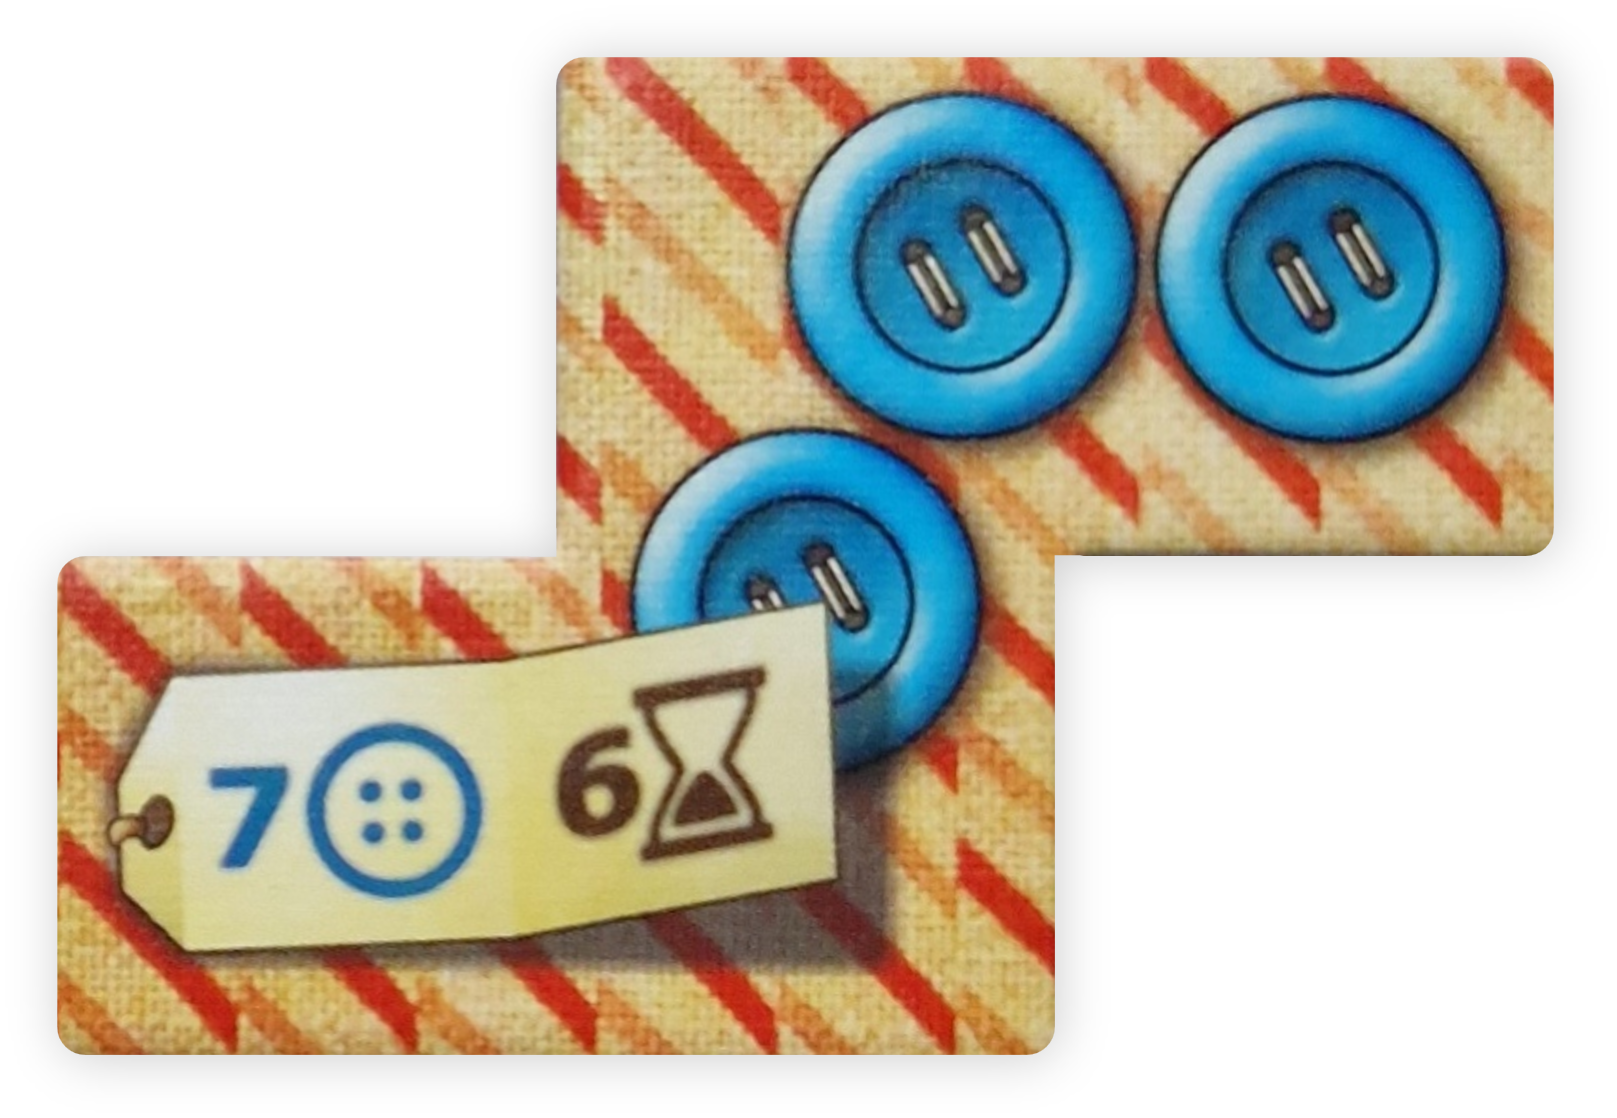
\includegraphics[width=0.2\textwidth]{res/pictures/assets/04-front.png}} & $4$  & $4$    & $7$              & $6$ & $3$ & $\frac{1}{8} = 0{,}125$        \\ \hline
    \adjustbox{valign=m, max width=0.2\textwidth, max height=0.1\textheight}{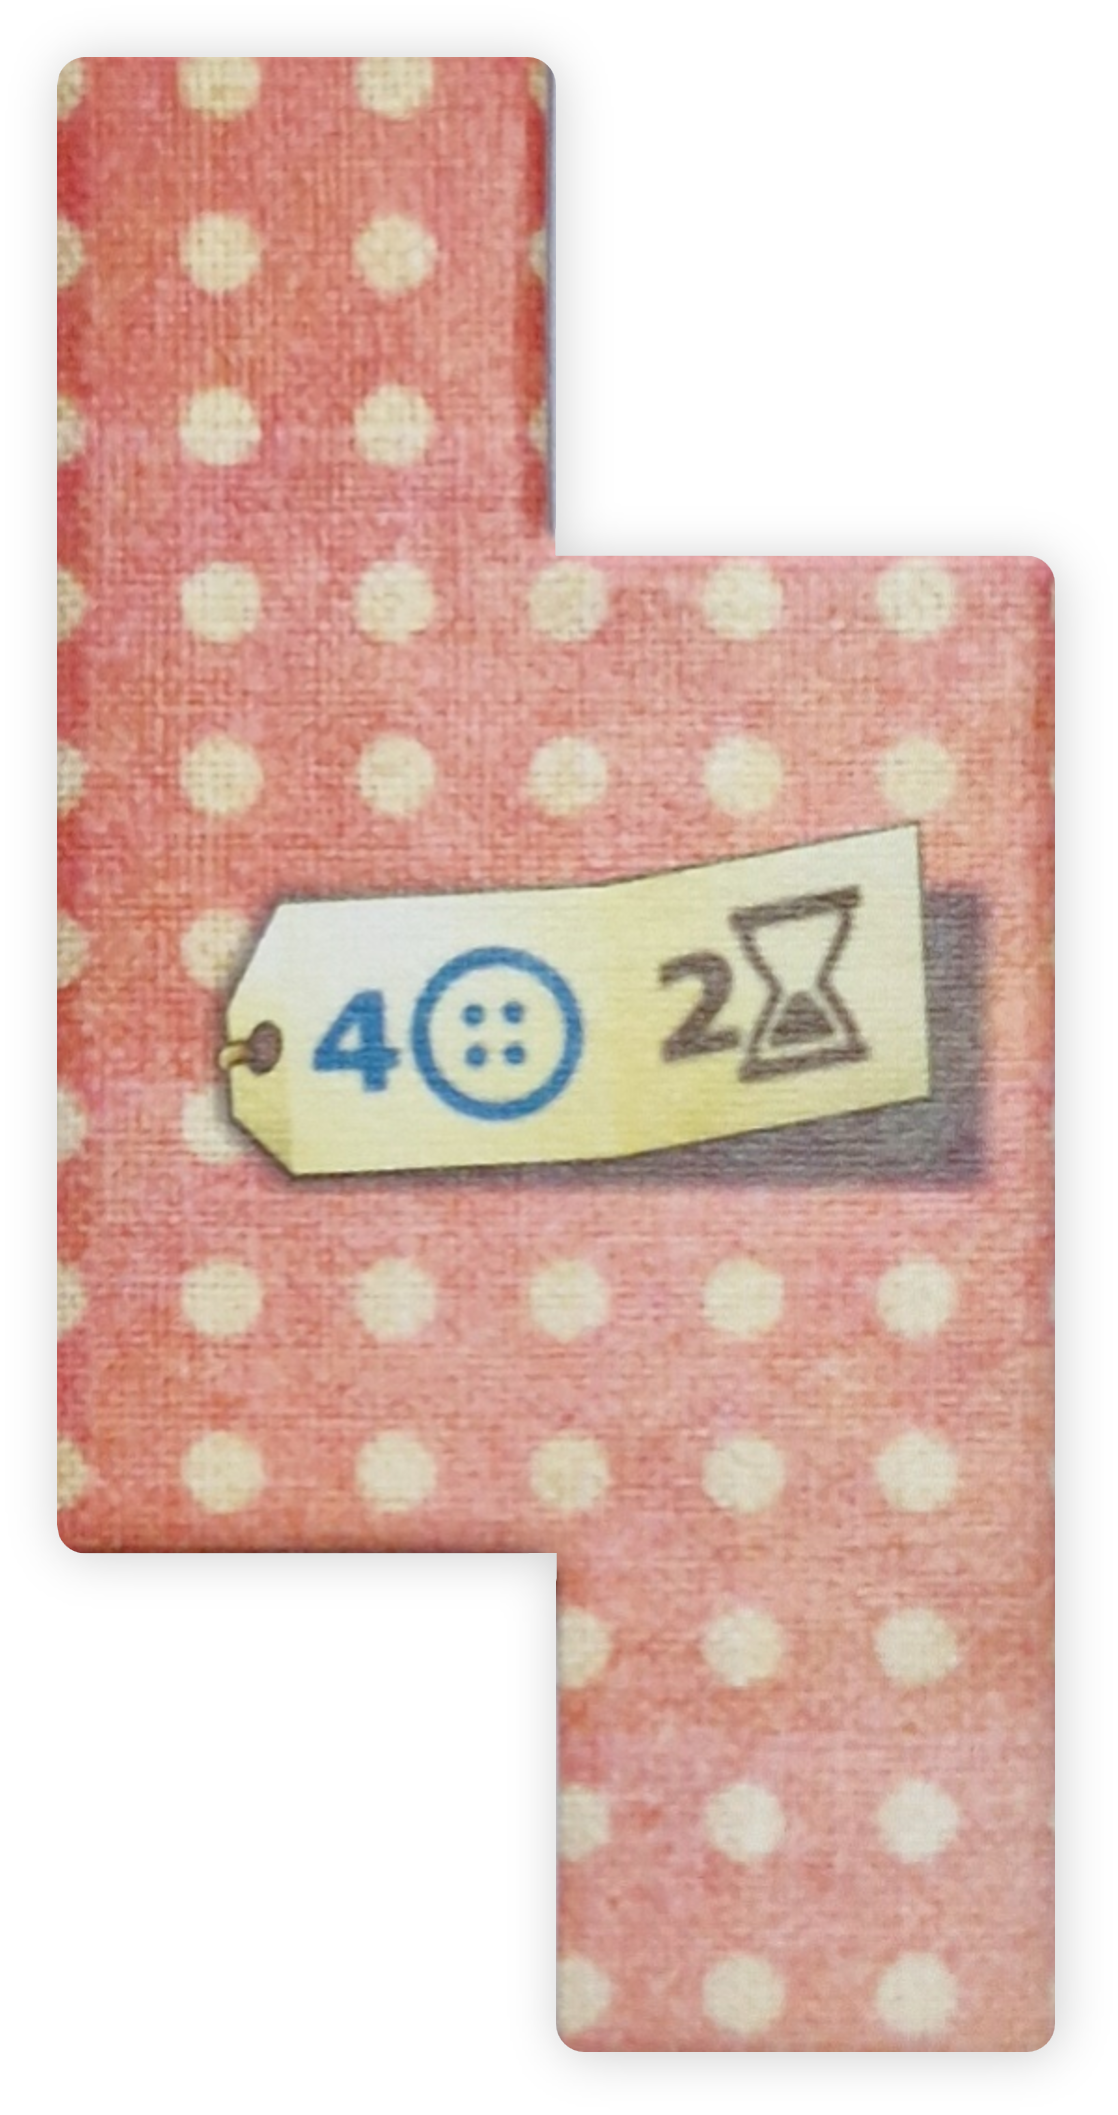
\includegraphics[width=0.2\textwidth]{res/pictures/assets/05-front.png}} & $5$  & $6$    & $4$              & $2$ & $0$ & $0$                            \\ \hline
    \adjustbox{valign=m, max width=0.2\textwidth, max height=0.1\textheight}{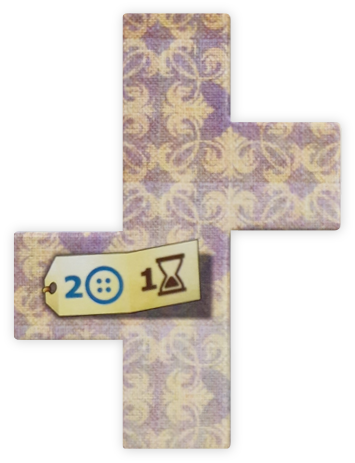
\includegraphics[width=0.2\textwidth]{res/pictures/assets/06-front.png}} & $6$  & $6$    & $2$              & $1$ & $0$ & $0$                            \\ \hline
    \adjustbox{valign=m, max width=0.2\textwidth, max height=0.1\textheight}{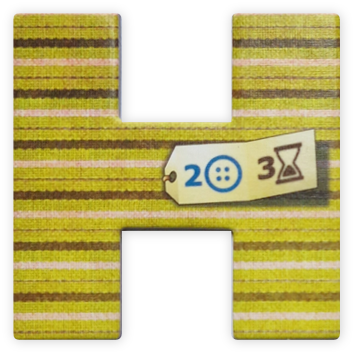
\includegraphics[width=0.2\textwidth]{res/pictures/assets/07-front.png}} & $7$  & $7$    & $2$              & $3$ & $0$ & $0$                            \\ \hline
    \adjustbox{valign=m, max width=0.2\textwidth, max height=0.1\textheight}{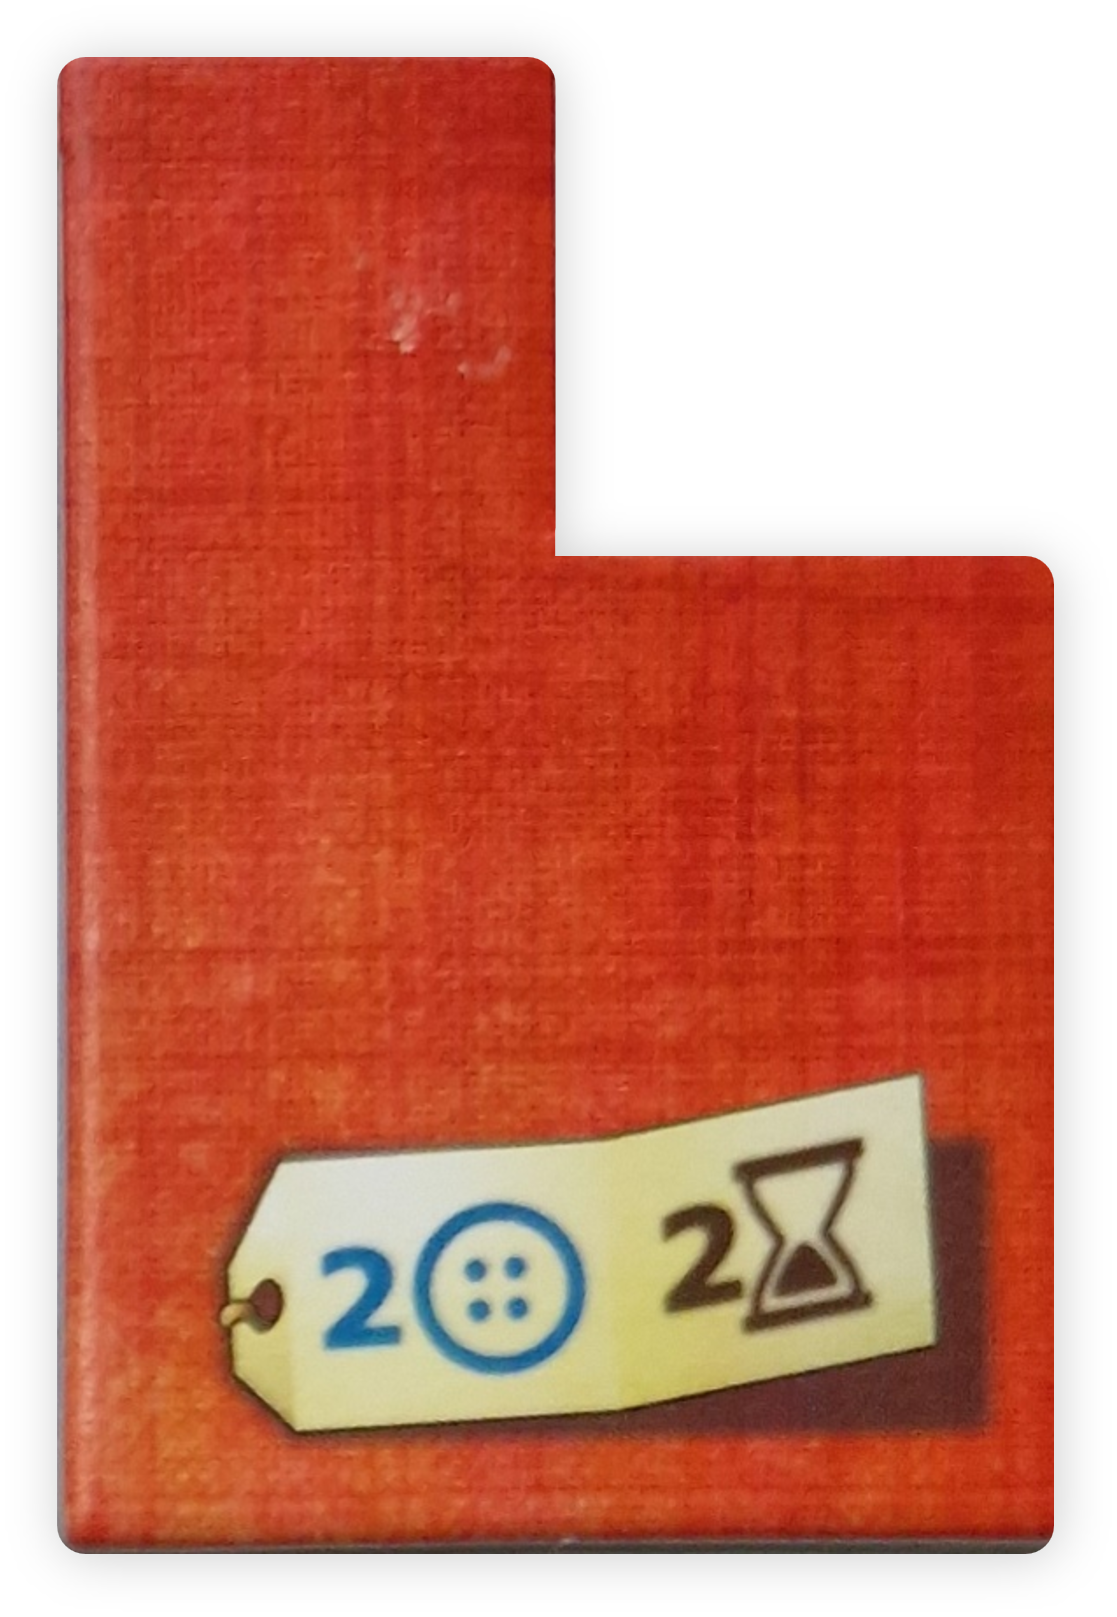
\includegraphics[width=0.2\textwidth]{res/pictures/assets/08-front.png}} & $8$  & $5$    & $2$              & $2$ & $0$ & $0$                            \\ \hline
    \adjustbox{valign=m, max width=0.2\textwidth, max height=0.1\textheight}{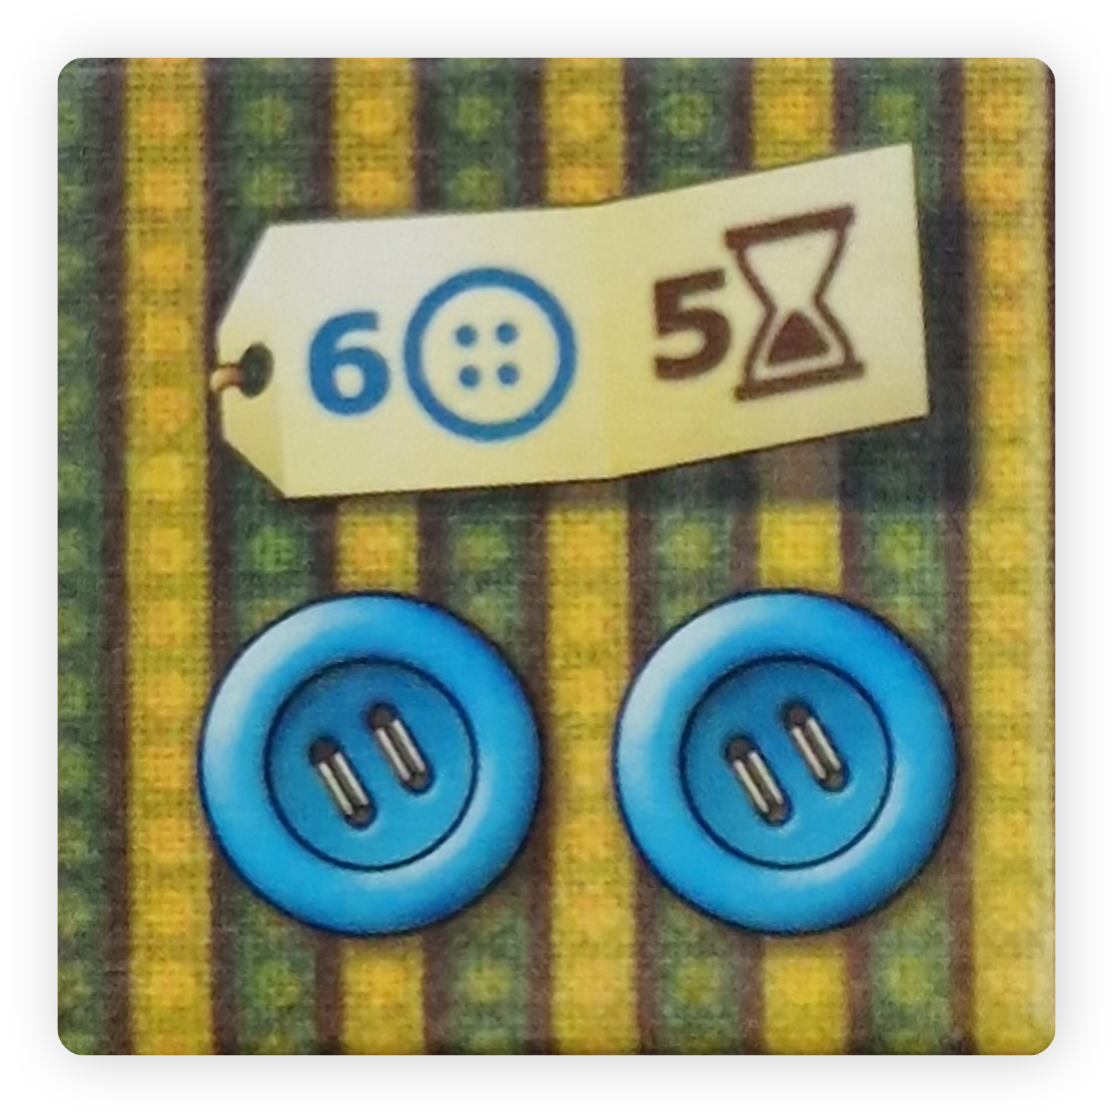
\includegraphics[width=0.2\textwidth]{res/pictures/assets/09-front.png}} & $9$  & $4$    & $6$              & $5$ & $2$ & $\frac{1}{10} = 0{,}1$         \\ \hline
    \adjustbox{valign=m, max width=0.2\textwidth, max height=0.1\textheight}{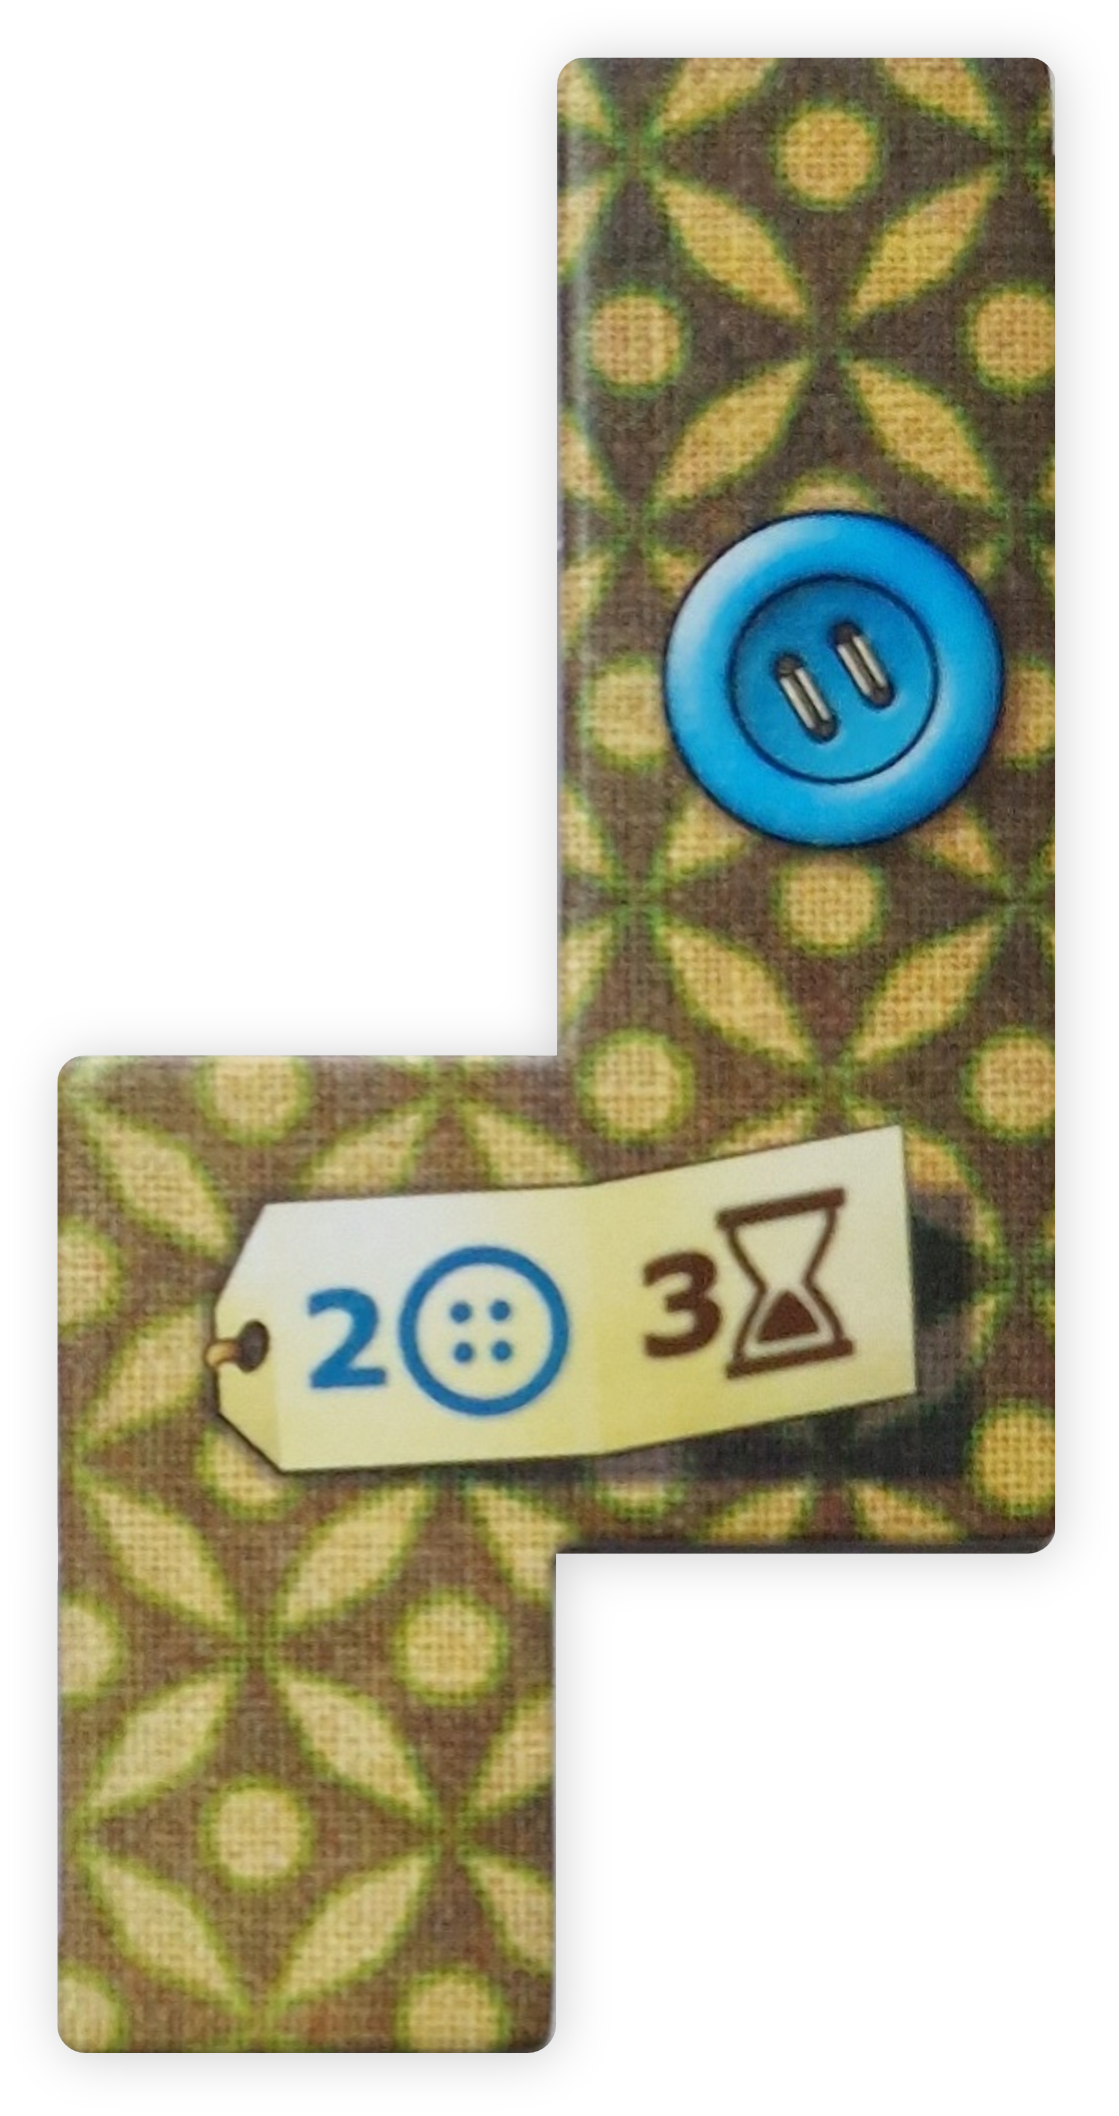
\includegraphics[width=0.2\textwidth]{res/pictures/assets/10-front.png}} & $10$ & $5$    & $2$              & $3$ & $1$ & $\frac{1}{15} \approx 0{,}067$ \\ \hline
    \adjustbox{valign=m, max width=0.2\textwidth, max height=0.1\textheight}{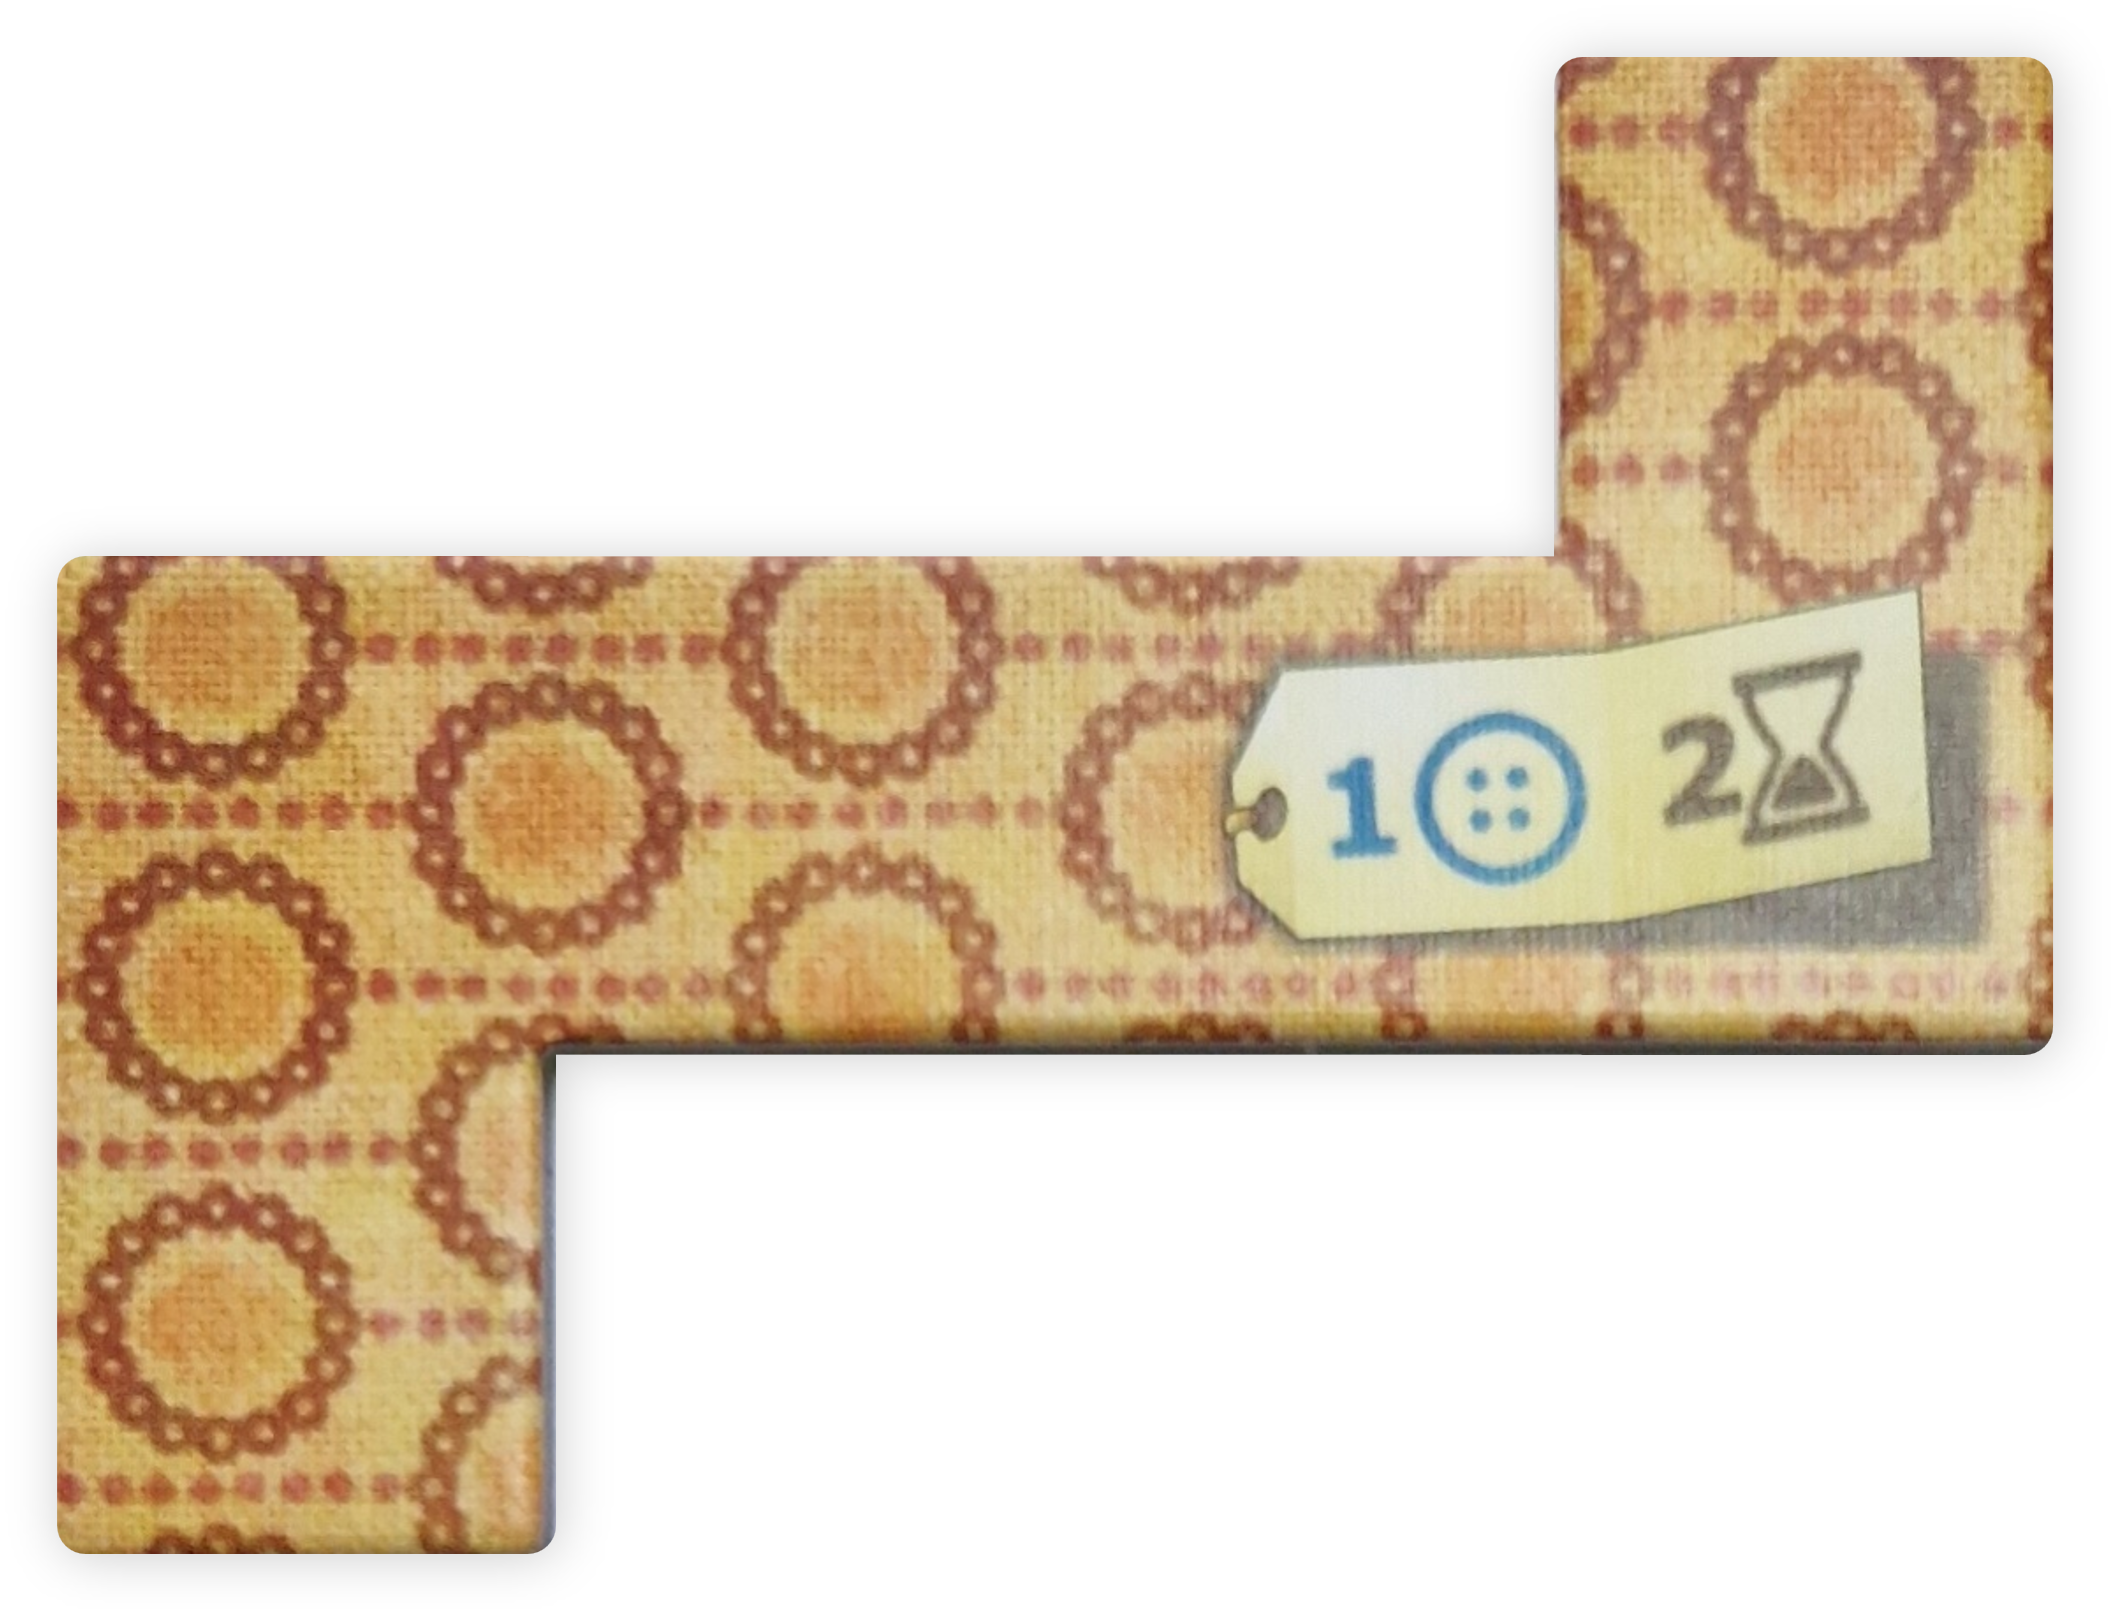
\includegraphics[width=0.2\textwidth]{res/pictures/assets/11-front.png}} & $11$ & $6$    & $1$              & $2$ & $0$ & $0$                            \\ \hline
    \adjustbox{valign=m, max width=0.2\textwidth, max height=0.1\textheight}{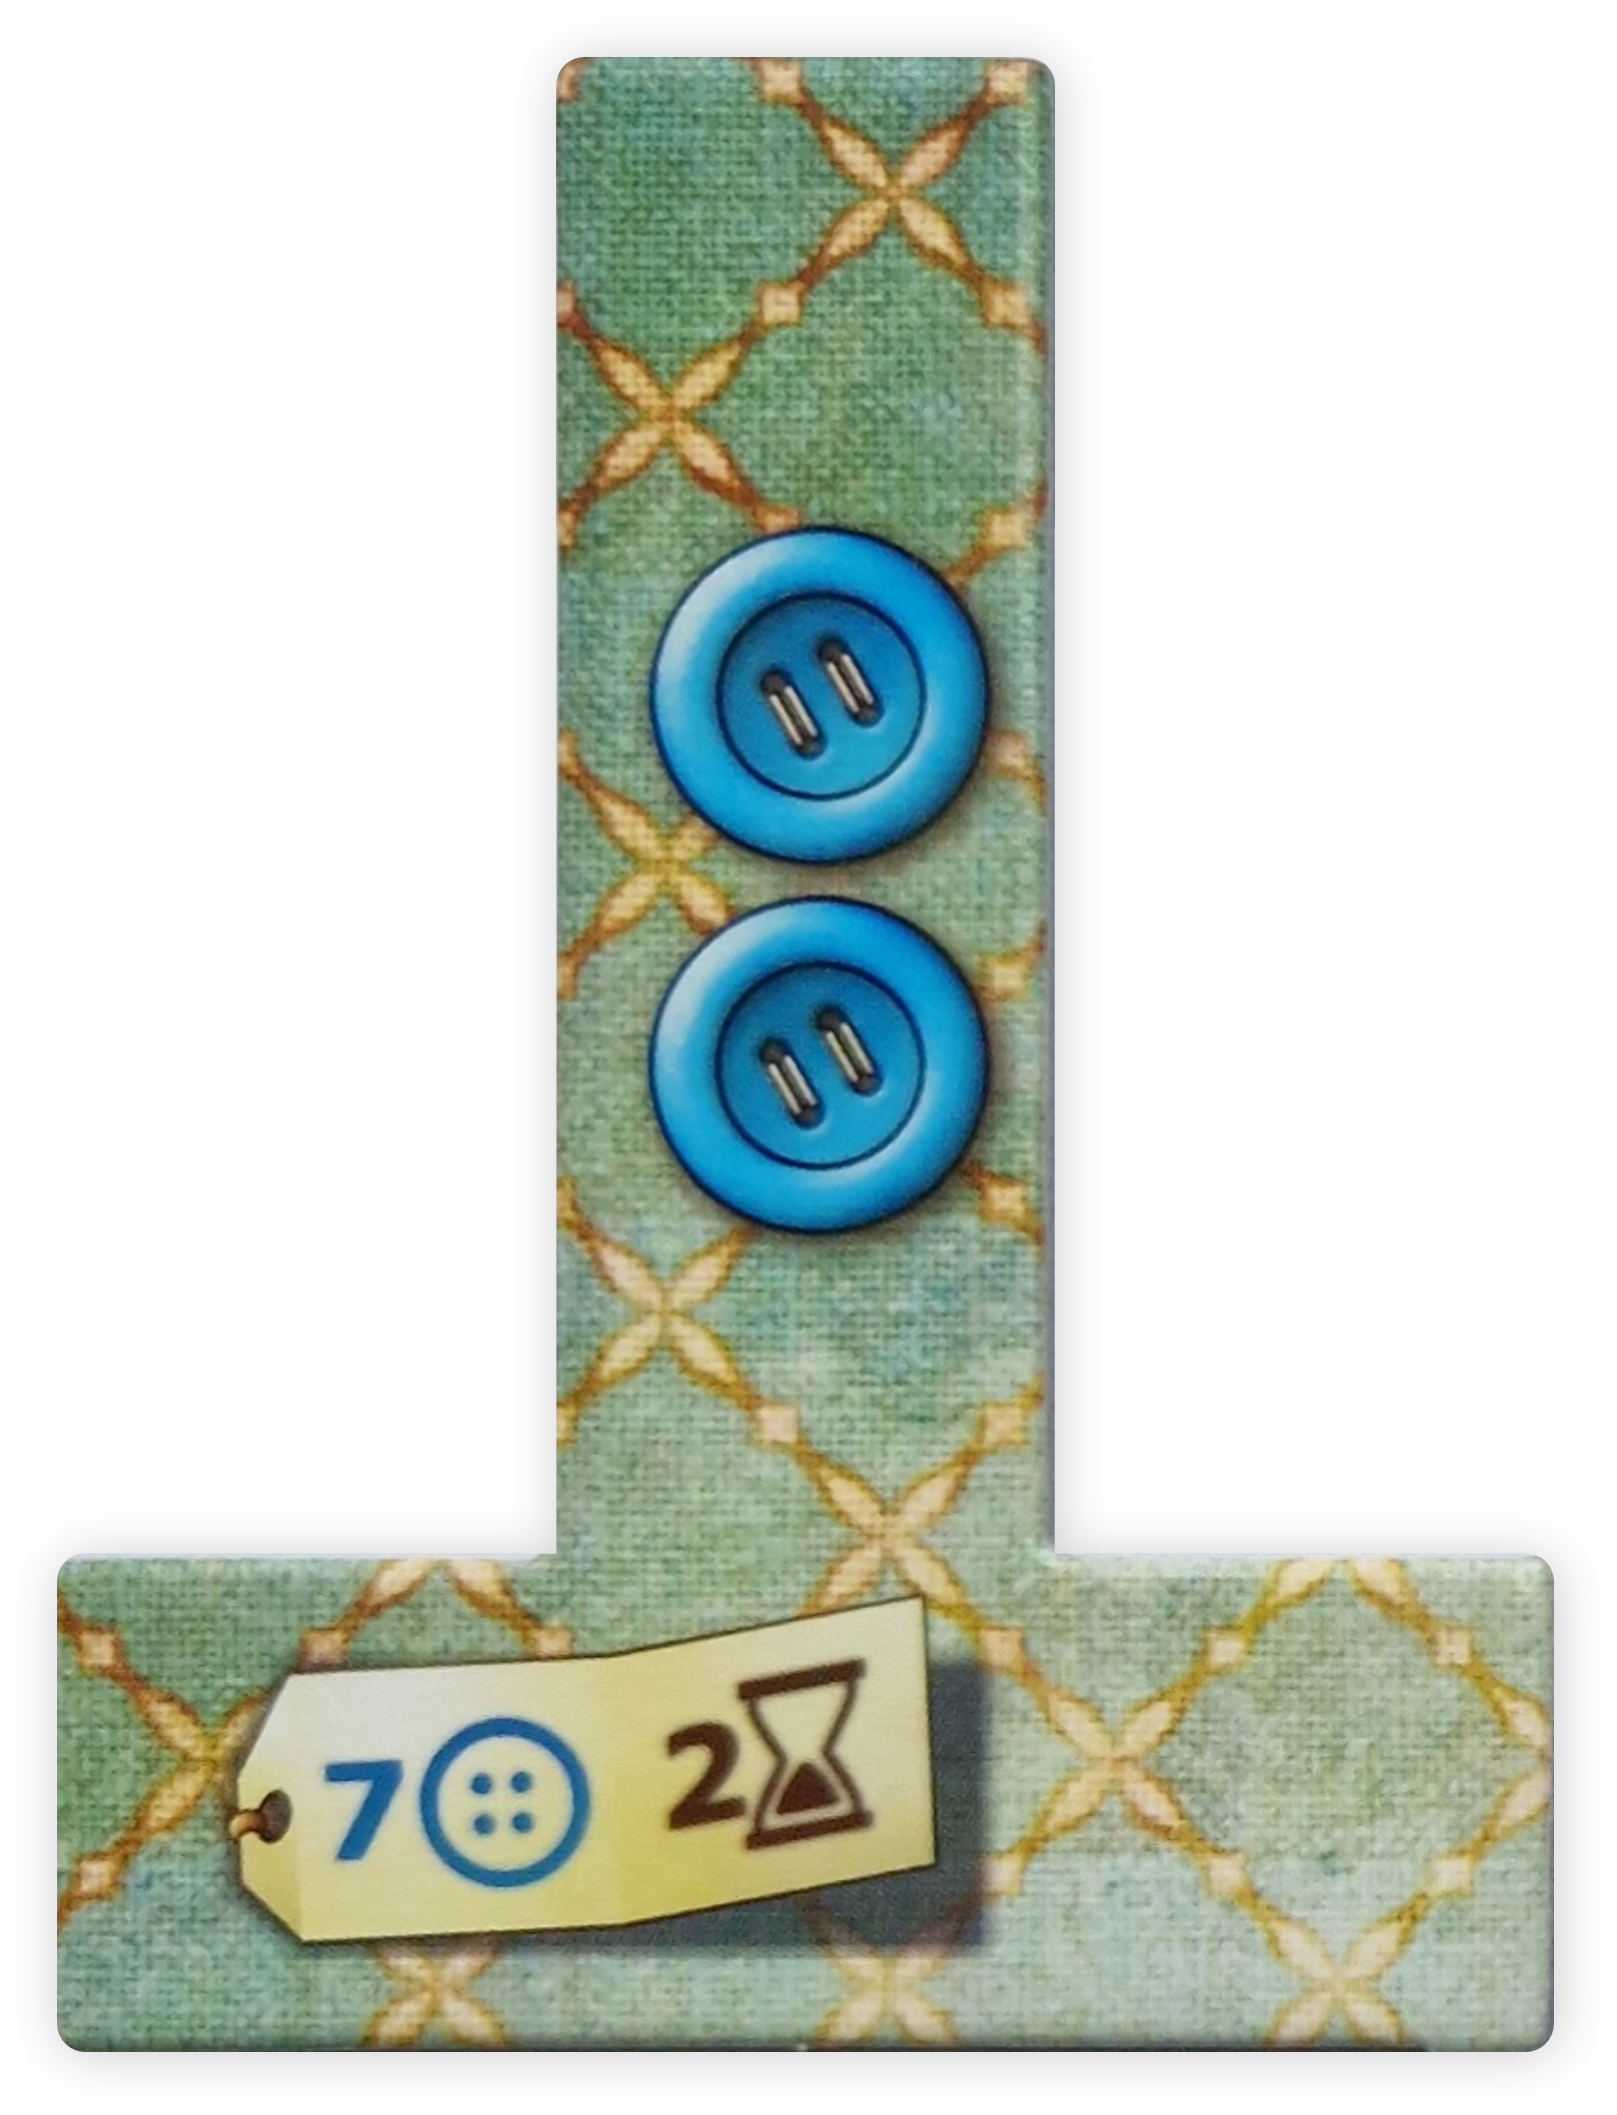
\includegraphics[width=0.2\textwidth]{res/pictures/assets/12-front.png}} & $12$ & $6$    & $7$              & $2$ & $2$ & $\frac{1}{16} \approx 0{,}167$ \\ \hline
    \adjustbox{valign=m, max width=0.2\textwidth, max height=0.1\textheight}{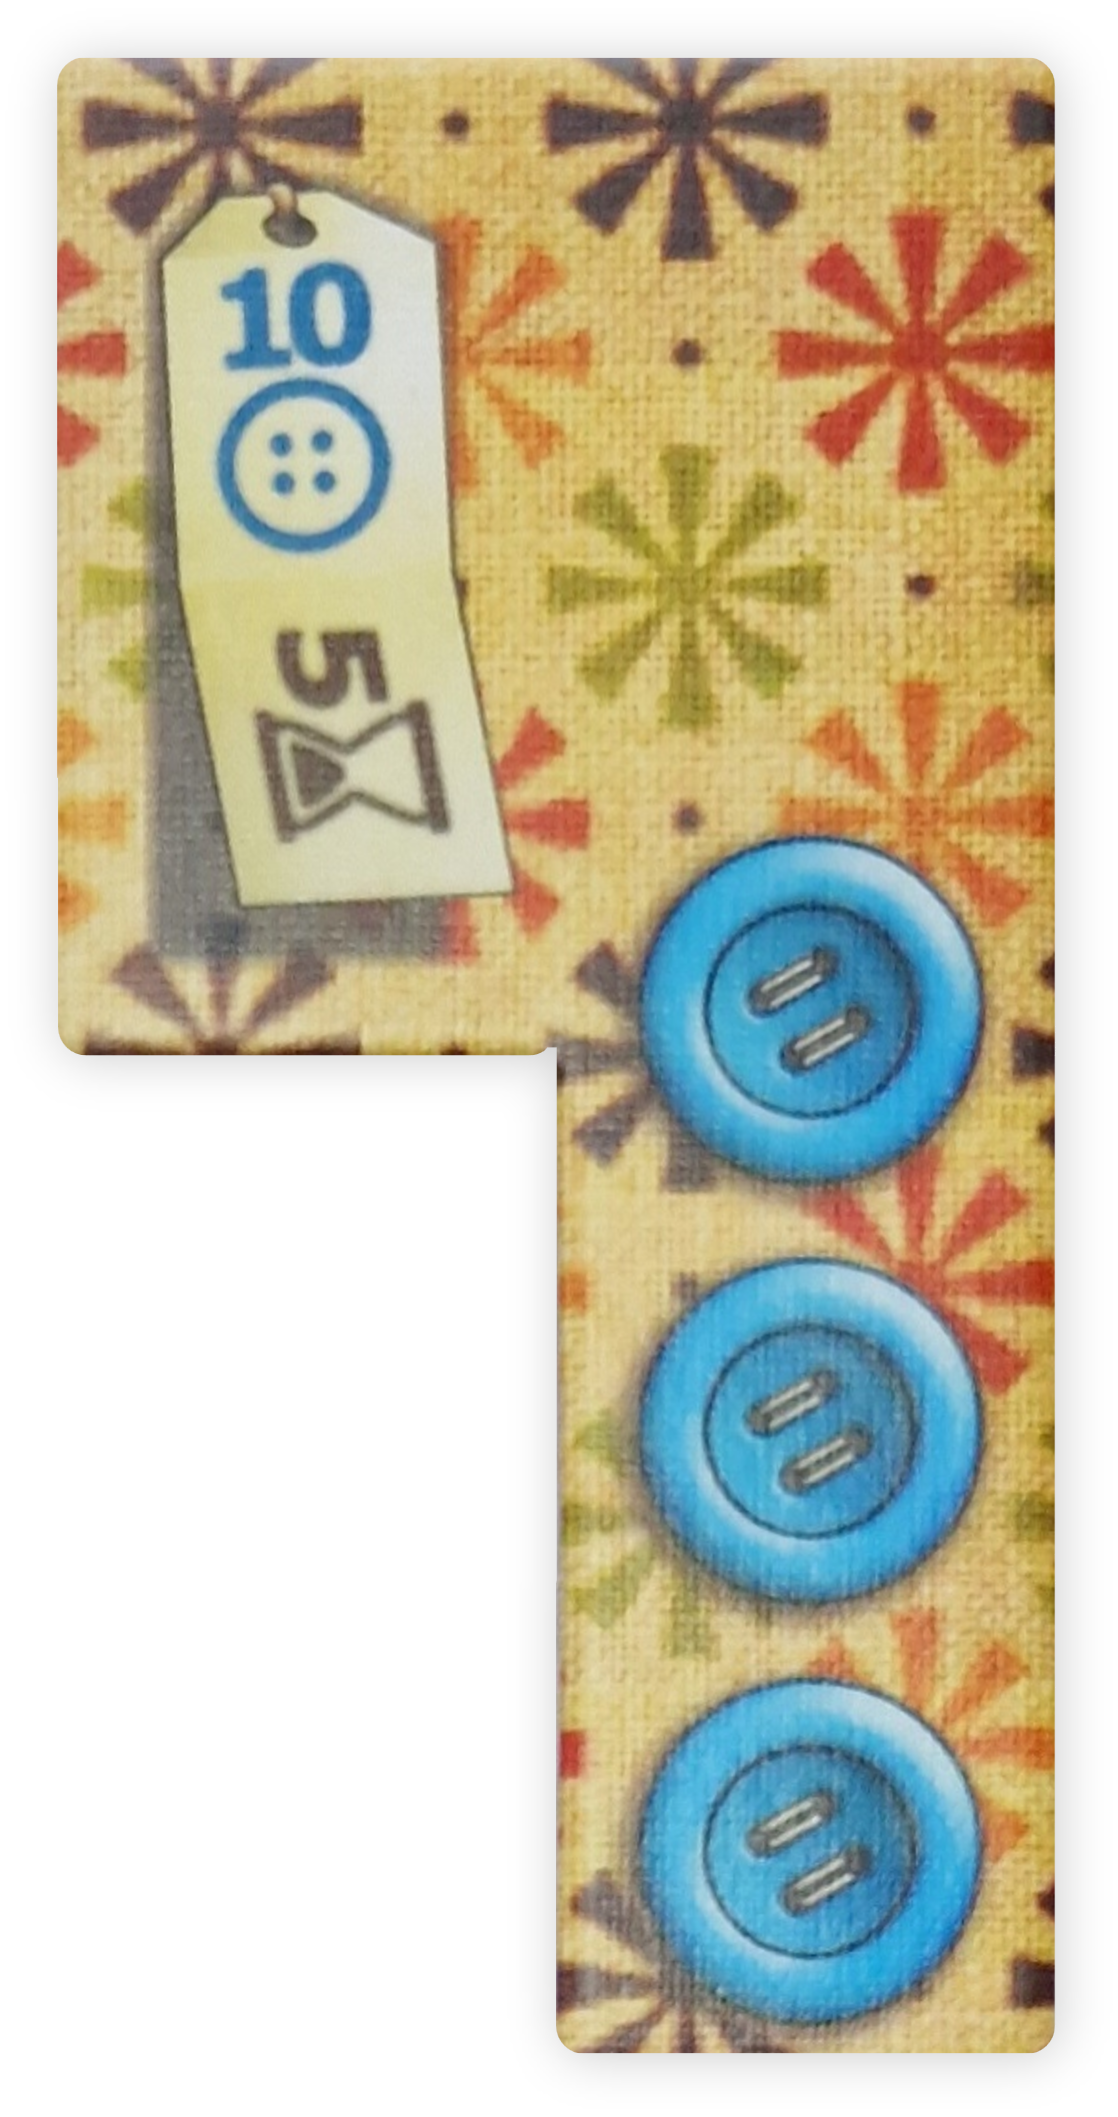
\includegraphics[width=0.2\textwidth]{res/pictures/assets/13-front.png}} & $13$ & $6$    & $10$             & $5$ & $3$ & $\frac{1}{10} = 0{,}1$         \\ \hline
    \adjustbox{valign=m, max width=0.2\textwidth, max height=0.1\textheight}{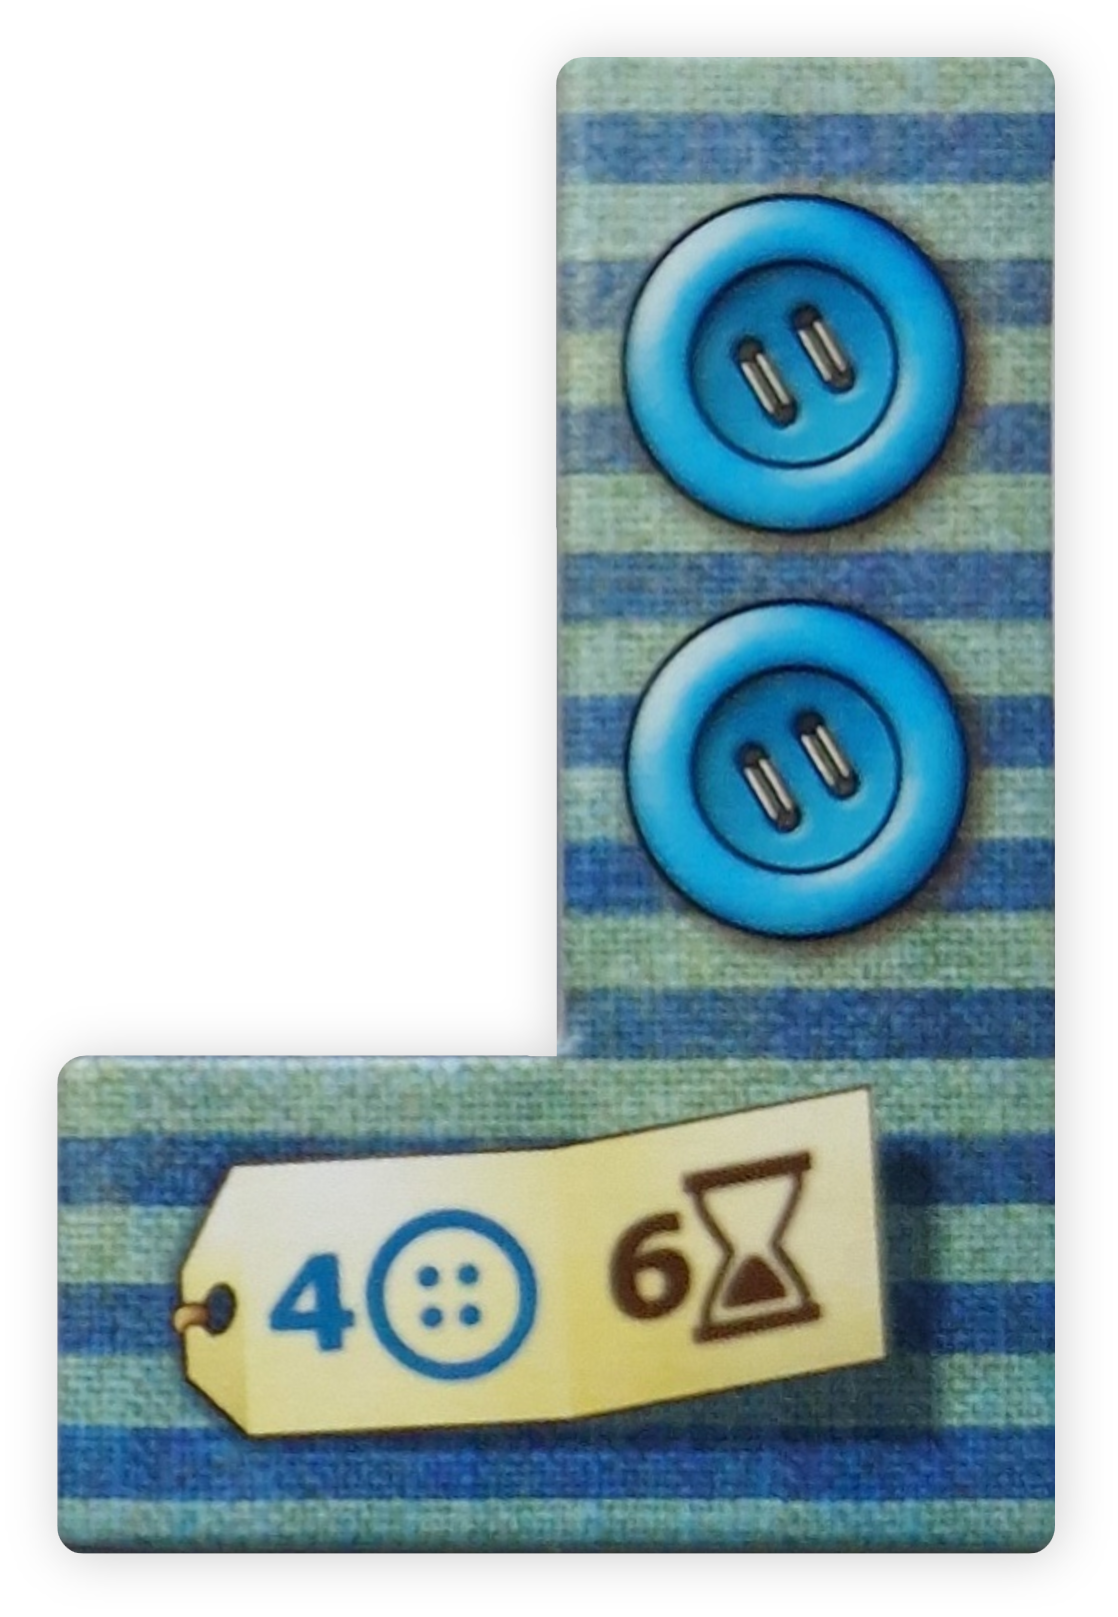
\includegraphics[width=0.2\textwidth]{res/pictures/assets/14-front.png}} & $14$ & $4$    & $4$              & $6$ & $2$ & $\frac{1}{12} \approx 0{,}083$ \\ \hline
    \adjustbox{valign=m, max width=0.2\textwidth, max height=0.1\textheight}{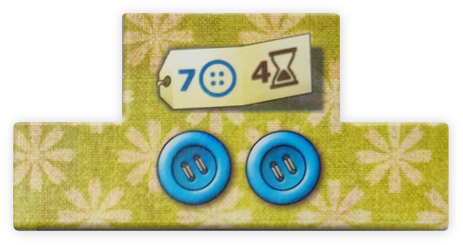
\includegraphics[width=0.2\textwidth]{res/pictures/assets/15-front.png}} & $15$ & $6$    & $7$              & $4$ & $2$ & $\frac{1}{12} \approx 0{,}083$ \\ \hline
    \adjustbox{valign=m, max width=0.2\textwidth, max height=0.1\textheight}{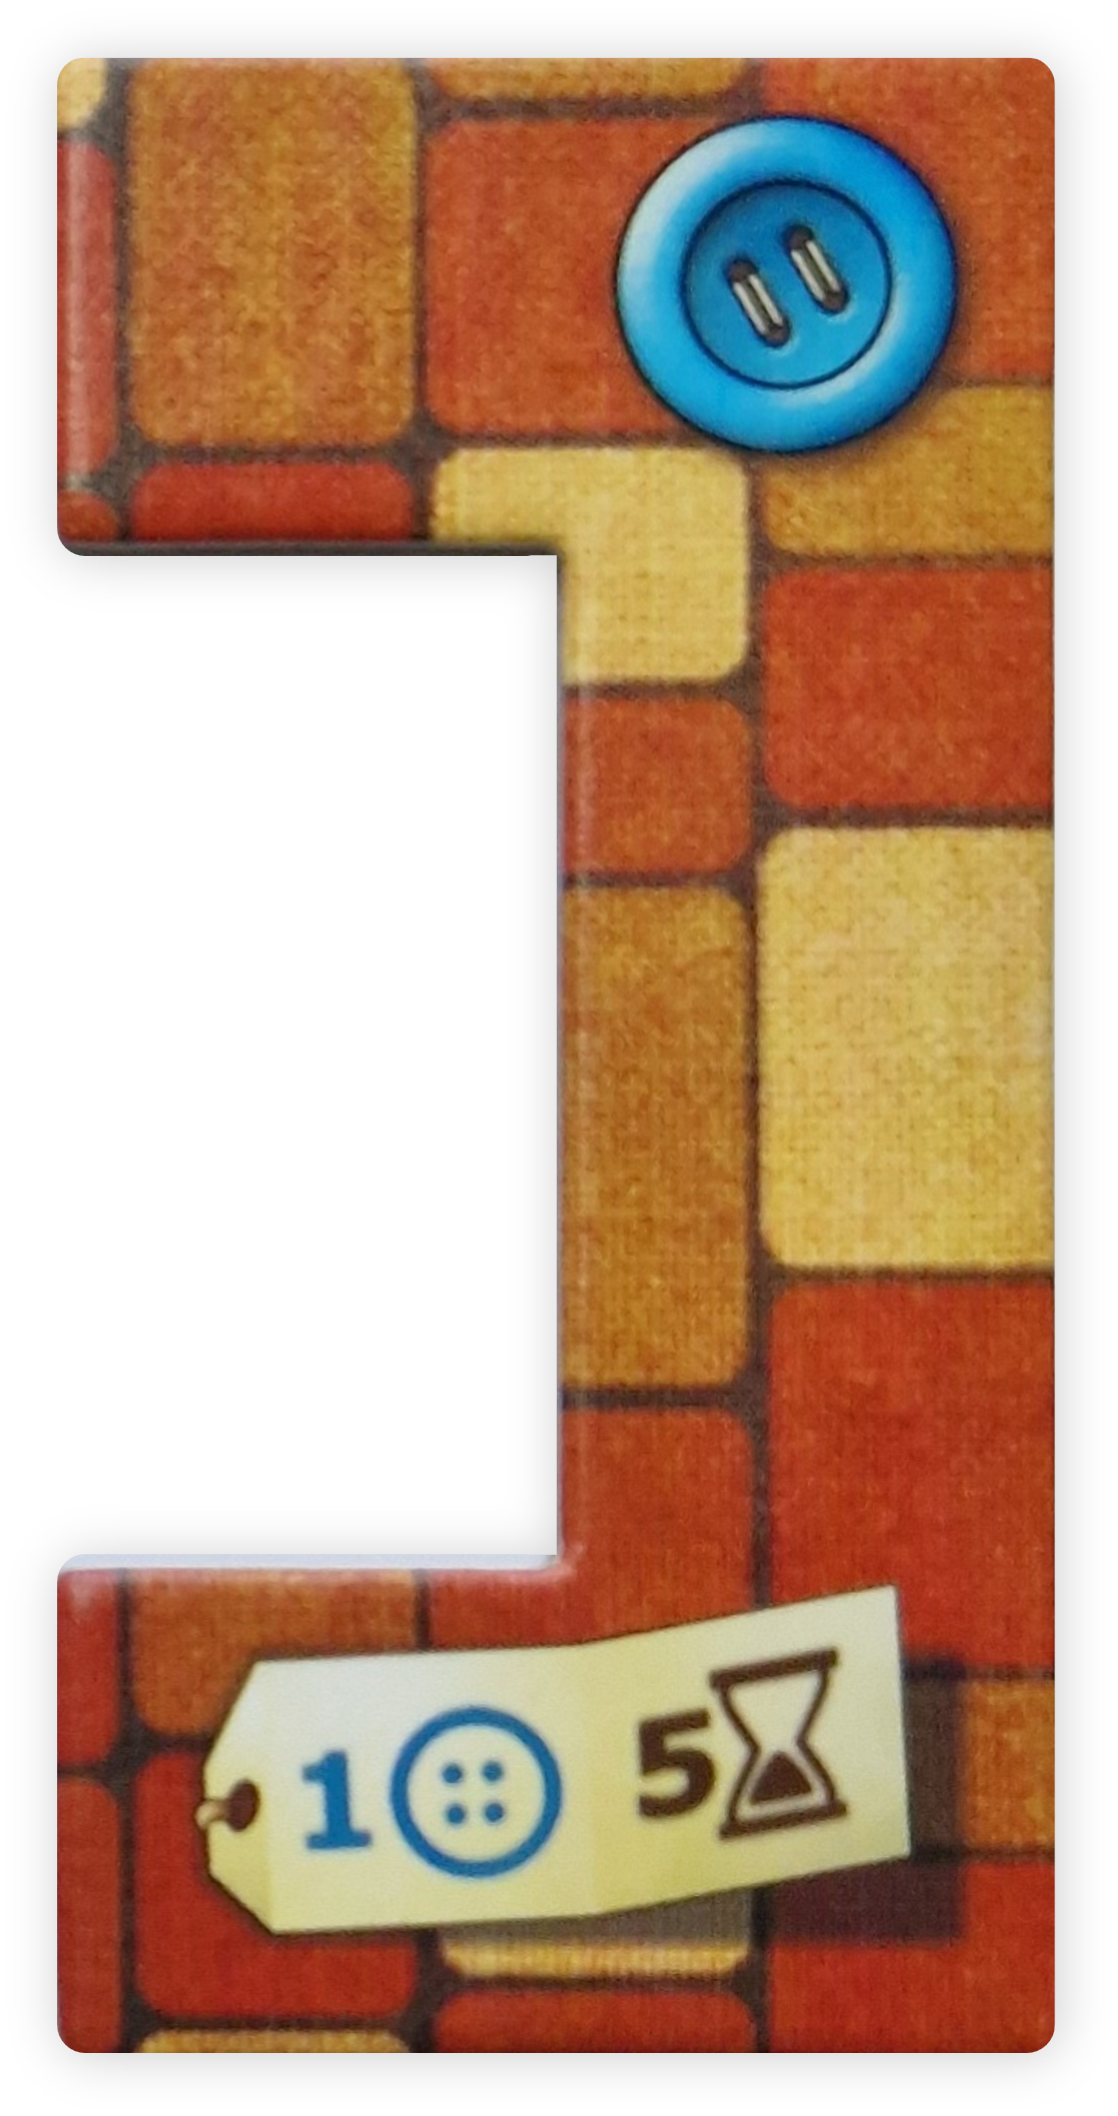
\includegraphics[width=0.2\textwidth]{res/pictures/assets/16-front.png}} & $16$ & $6$    & $1$              & $5$ & $1$ & $\frac{1}{30} \approx 0{,}033$ \\ \hline
    \adjustbox{valign=m, max width=0.2\textwidth, max height=0.1\textheight}{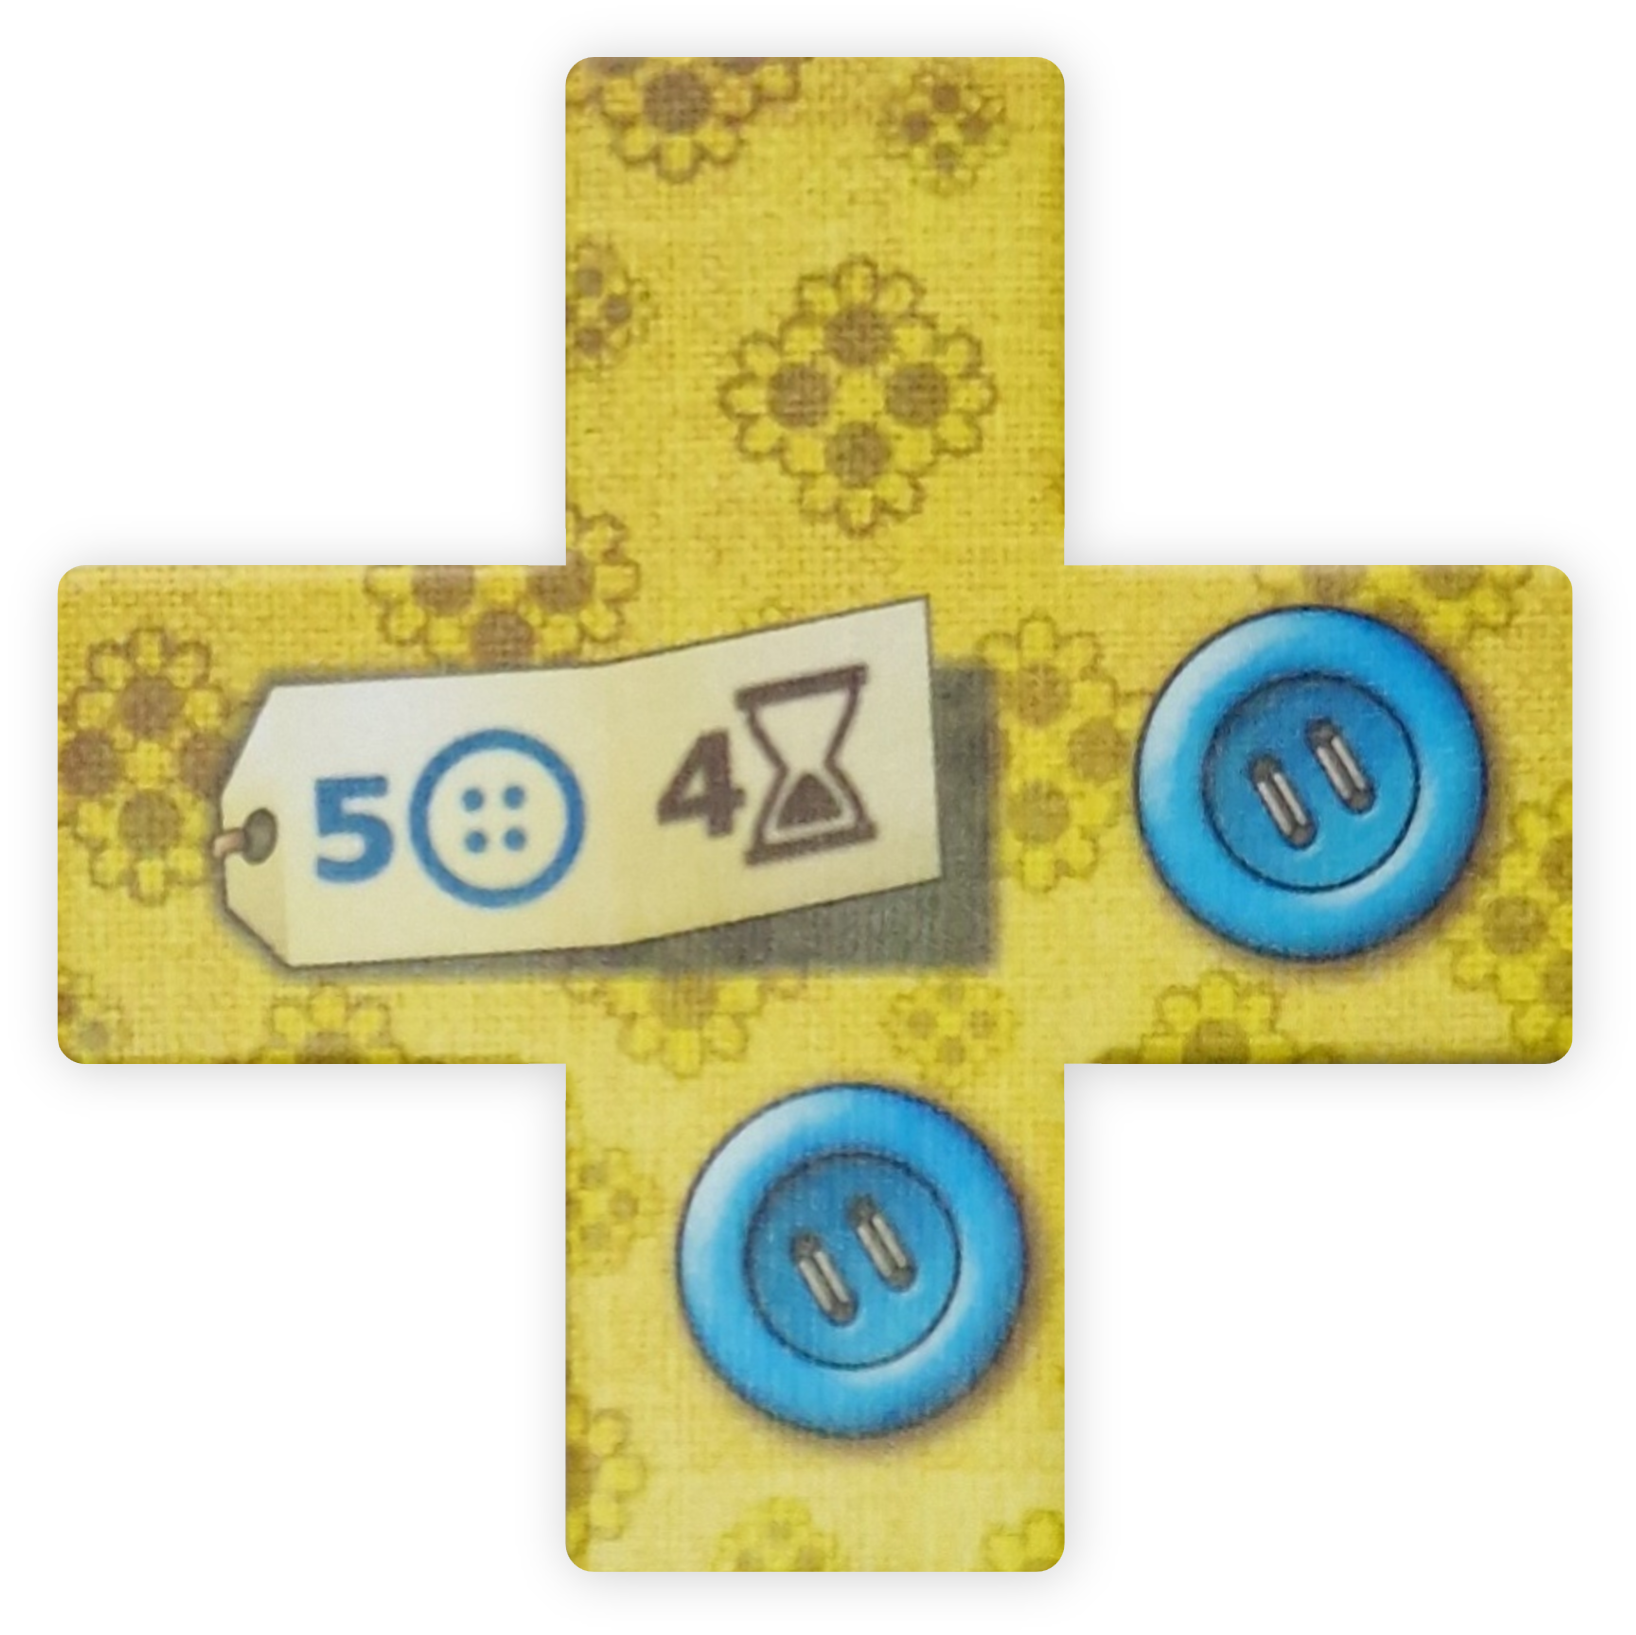
\includegraphics[width=0.2\textwidth]{res/pictures/assets/17-front.png}} & $17$ & $5$    & $5$              & $4$ & $2$ & $\frac{1}{10} = 0{,}1$         \\ \hline
    \adjustbox{valign=m, max width=0.2\textwidth, max height=0.1\textheight}{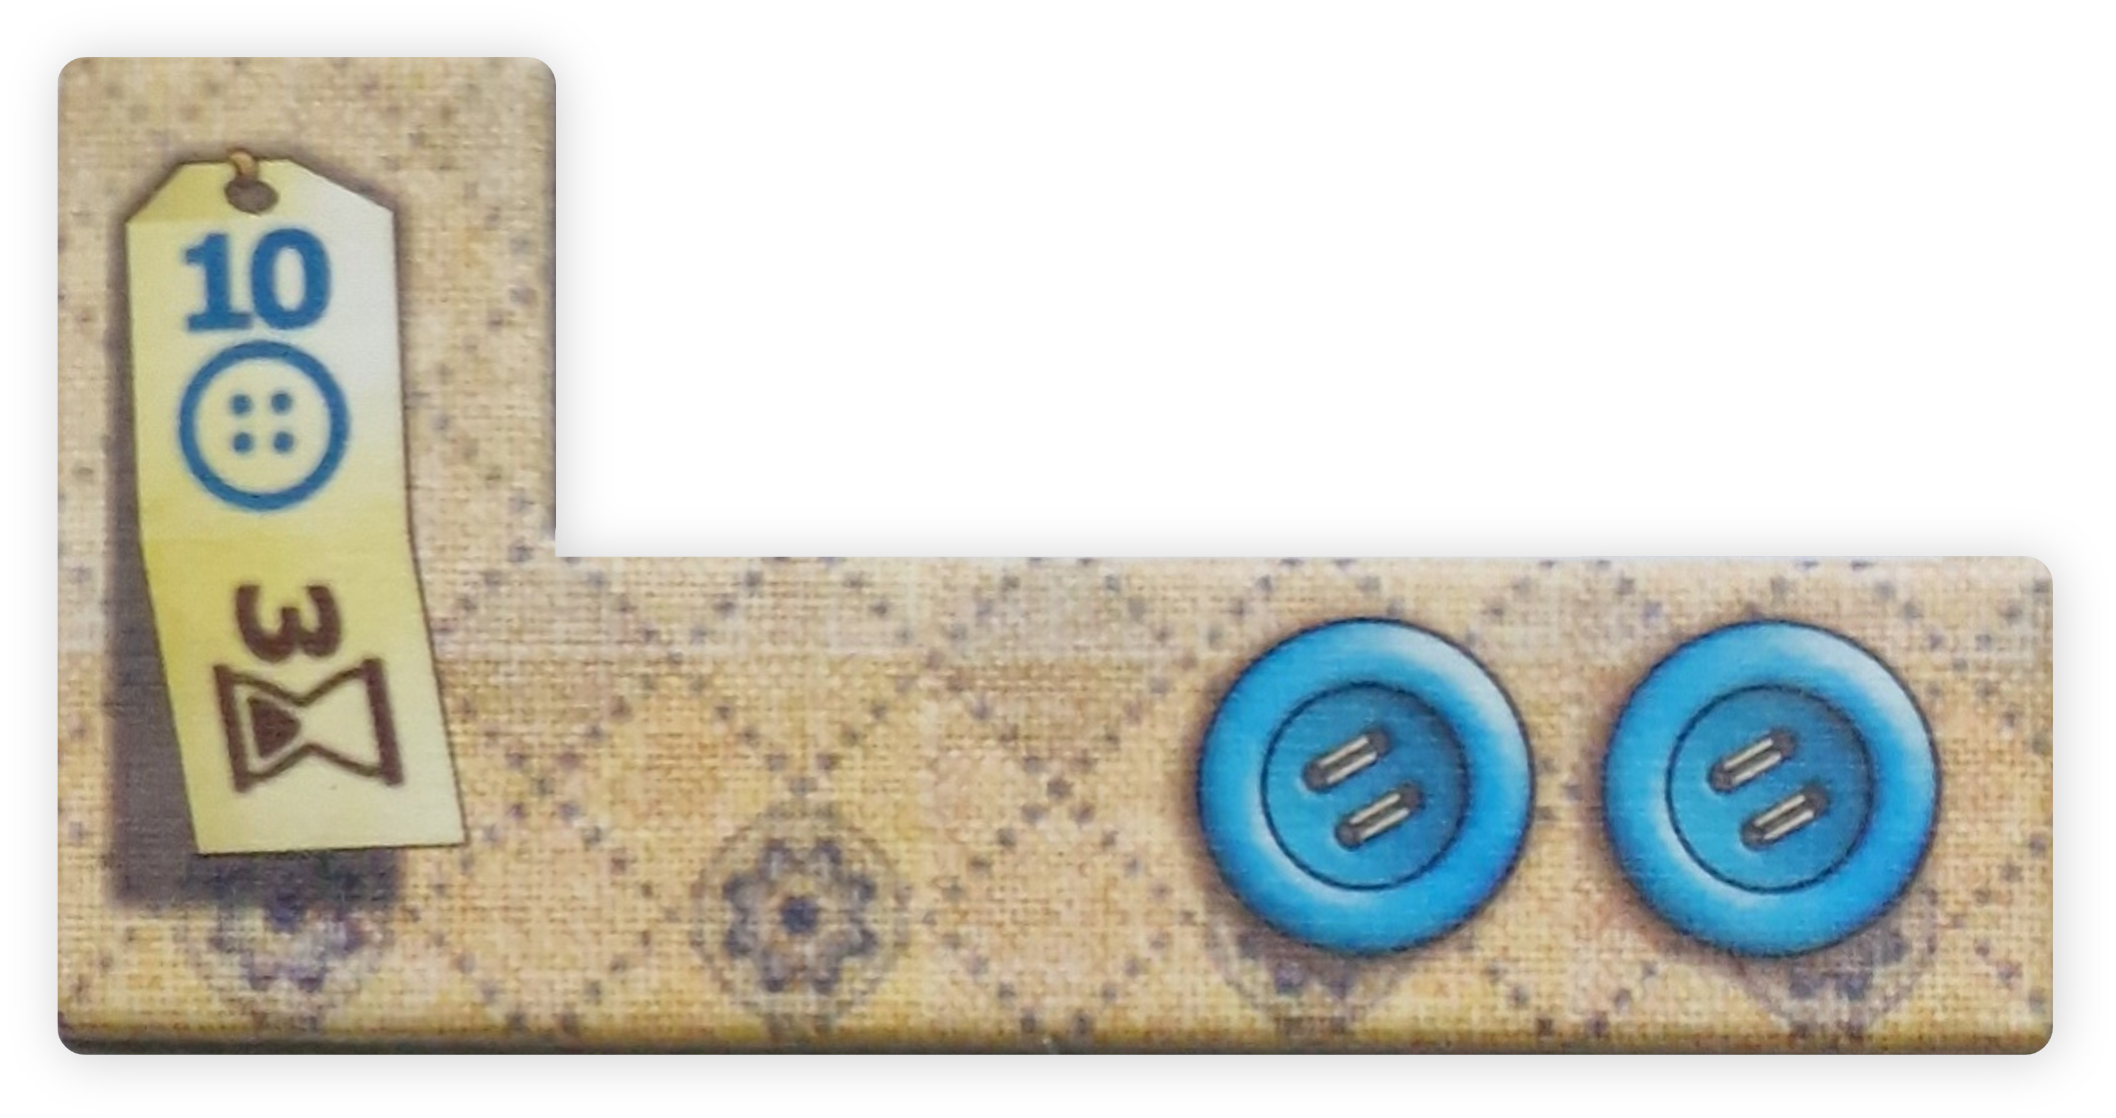
\includegraphics[width=0.2\textwidth]{res/pictures/assets/18-front.png}} & $18$ & $5$    & $10$             & $3$ & $2$ & $\frac{2}{15} \approx 0{,}133$ \\ \hline
    \adjustbox{valign=m, max width=0.2\textwidth, max height=0.1\textheight}{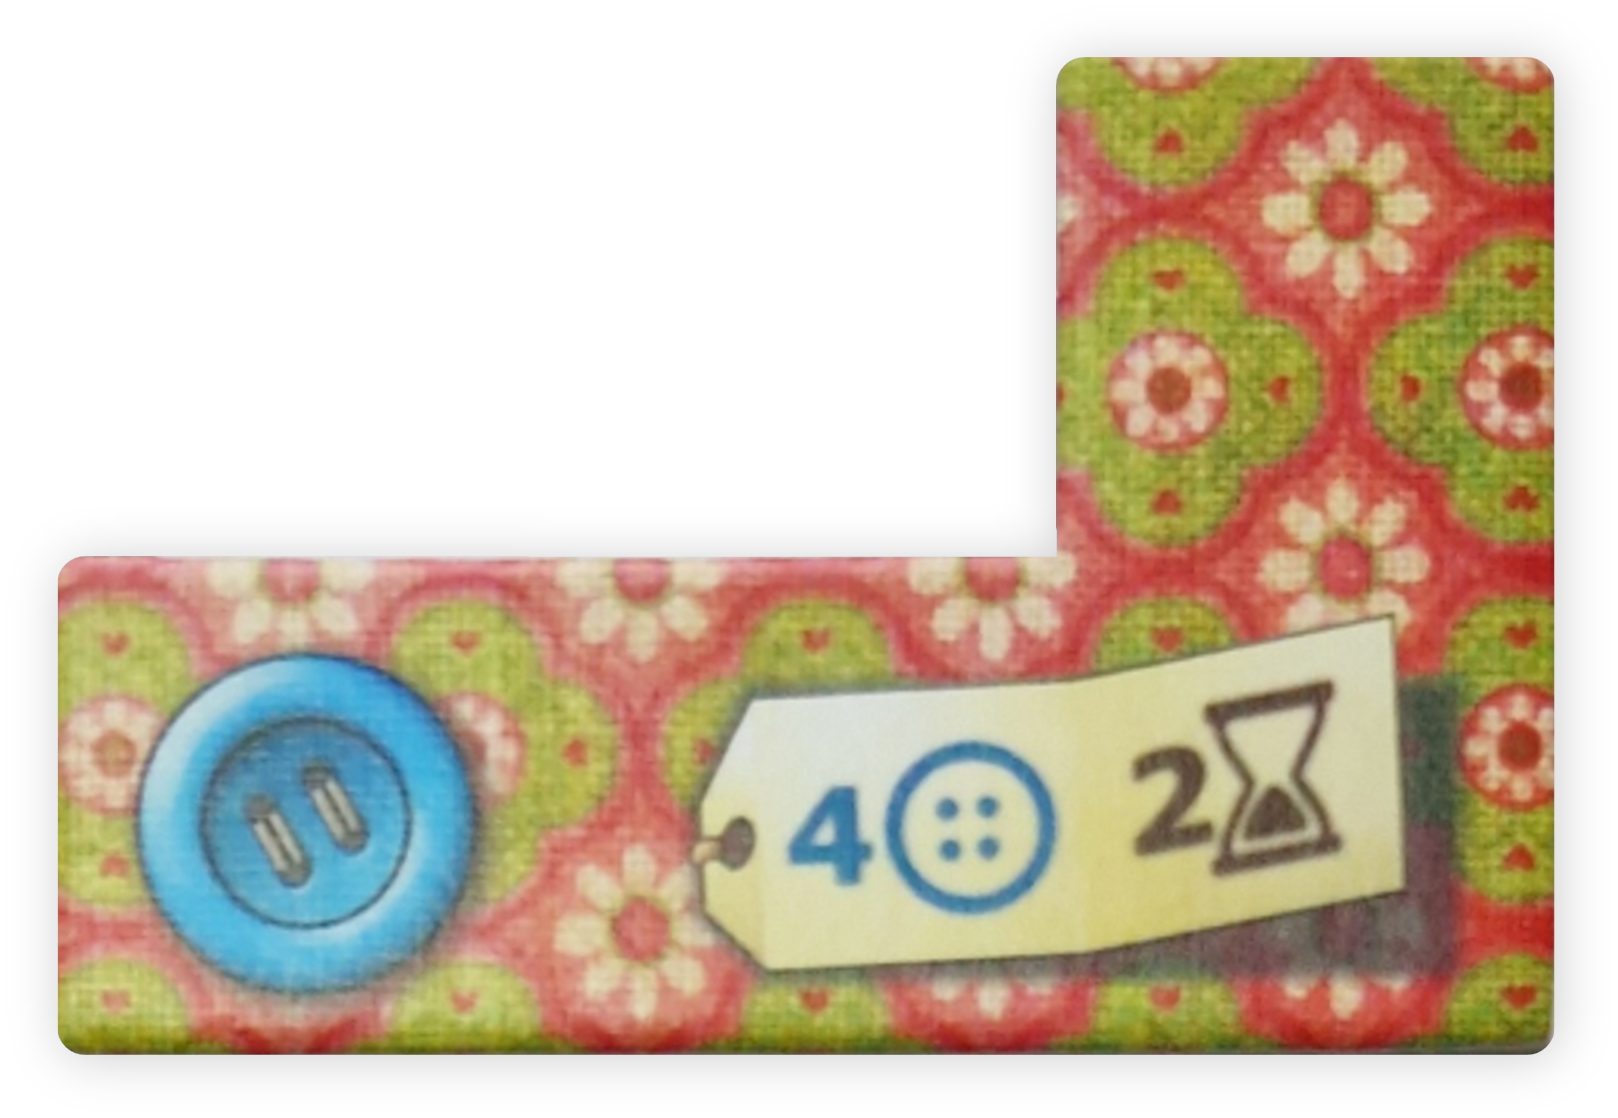
\includegraphics[width=0.2\textwidth]{res/pictures/assets/19-front.png}} & $19$ & $4$    & $4$              & $2$ & $1$ & $\frac{1}{8} = 0{,}125$        \\ \hline
    \adjustbox{valign=m, max width=0.2\textwidth, max height=0.1\textheight}{\includegraphics[width=0.2\textwidth]{res/pictures/assets/20-front.png}} & $20$ & $7$    & $1$              & $4$ & $1$ & $\frac{1}{28} \approx 0{,}036$ \\ \hline
    \adjustbox{valign=m, max width=0.2\textwidth, max height=0.1\textheight}{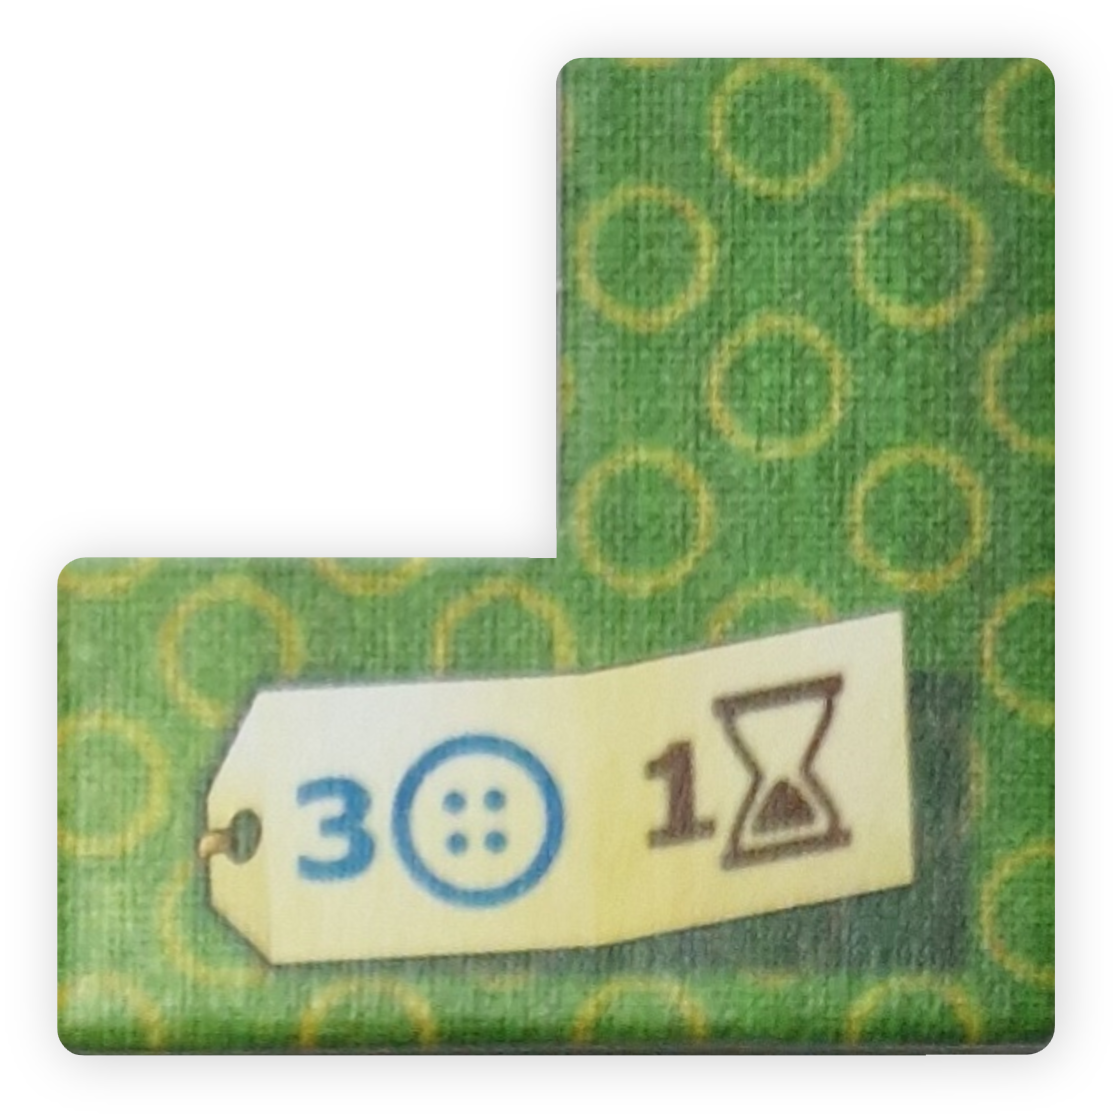
\includegraphics[width=0.2\textwidth]{res/pictures/assets/21-front.png}} & $21$ & $3$    & $1$              & $3$ & $0$ & $0$                            \\ \hline
    \adjustbox{valign=m, max width=0.2\textwidth, max height=0.1\textheight}{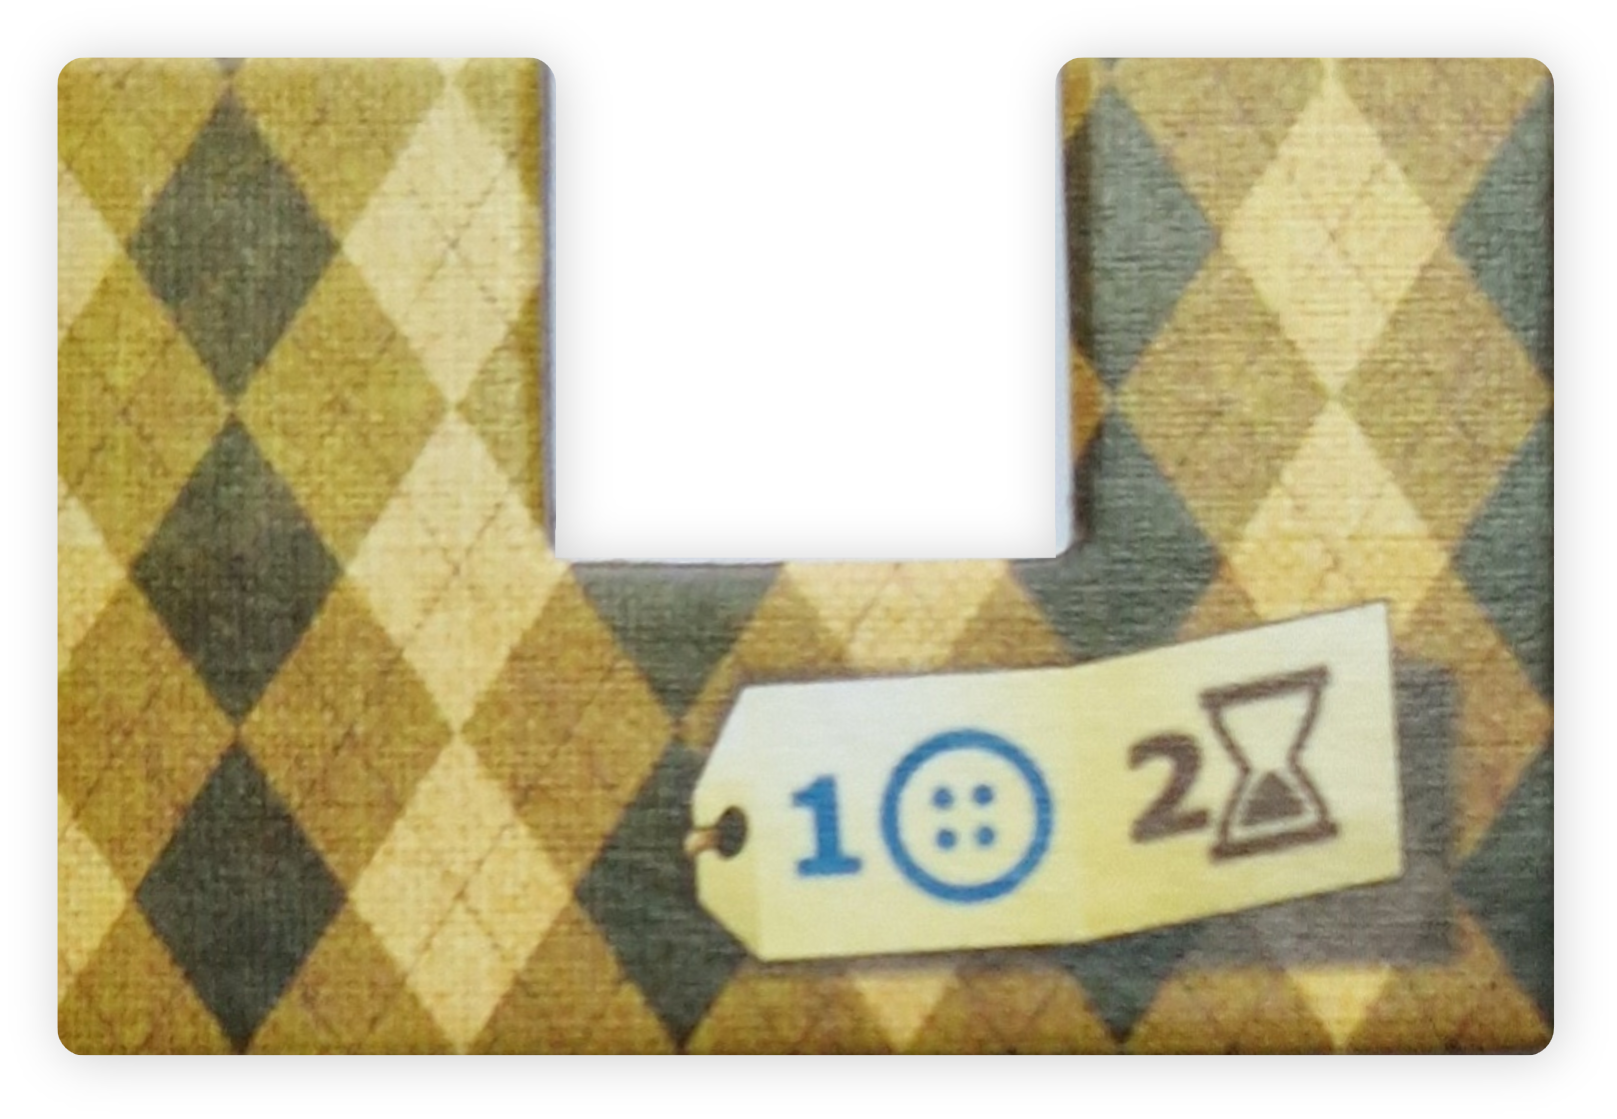
\includegraphics[width=0.2\textwidth]{res/pictures/assets/22-front.png}} & $22$ & $5$    & $1$              & $2$ & $0$ & $0$                            \\ \hline
    \adjustbox{valign=m, max width=0.2\textwidth, max height=0.1\textheight}{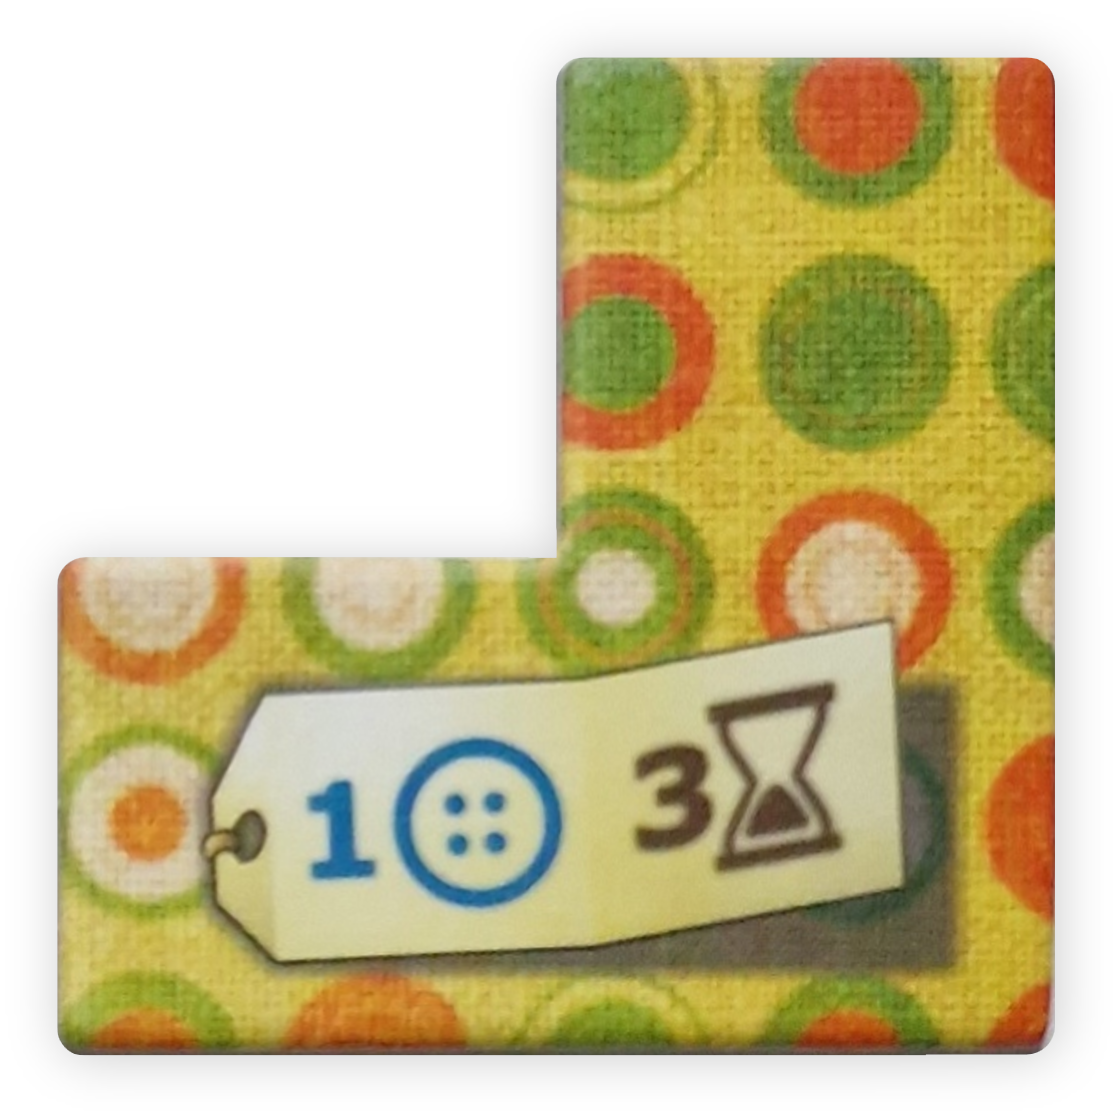
\includegraphics[width=0.2\textwidth]{res/pictures/assets/23-front.png}} & $23$ & $3$    & $3$              & $1$ & $0$ & $0$                            \\ \hline
    \adjustbox{valign=m, max width=0.2\textwidth, max height=0.1\textheight}{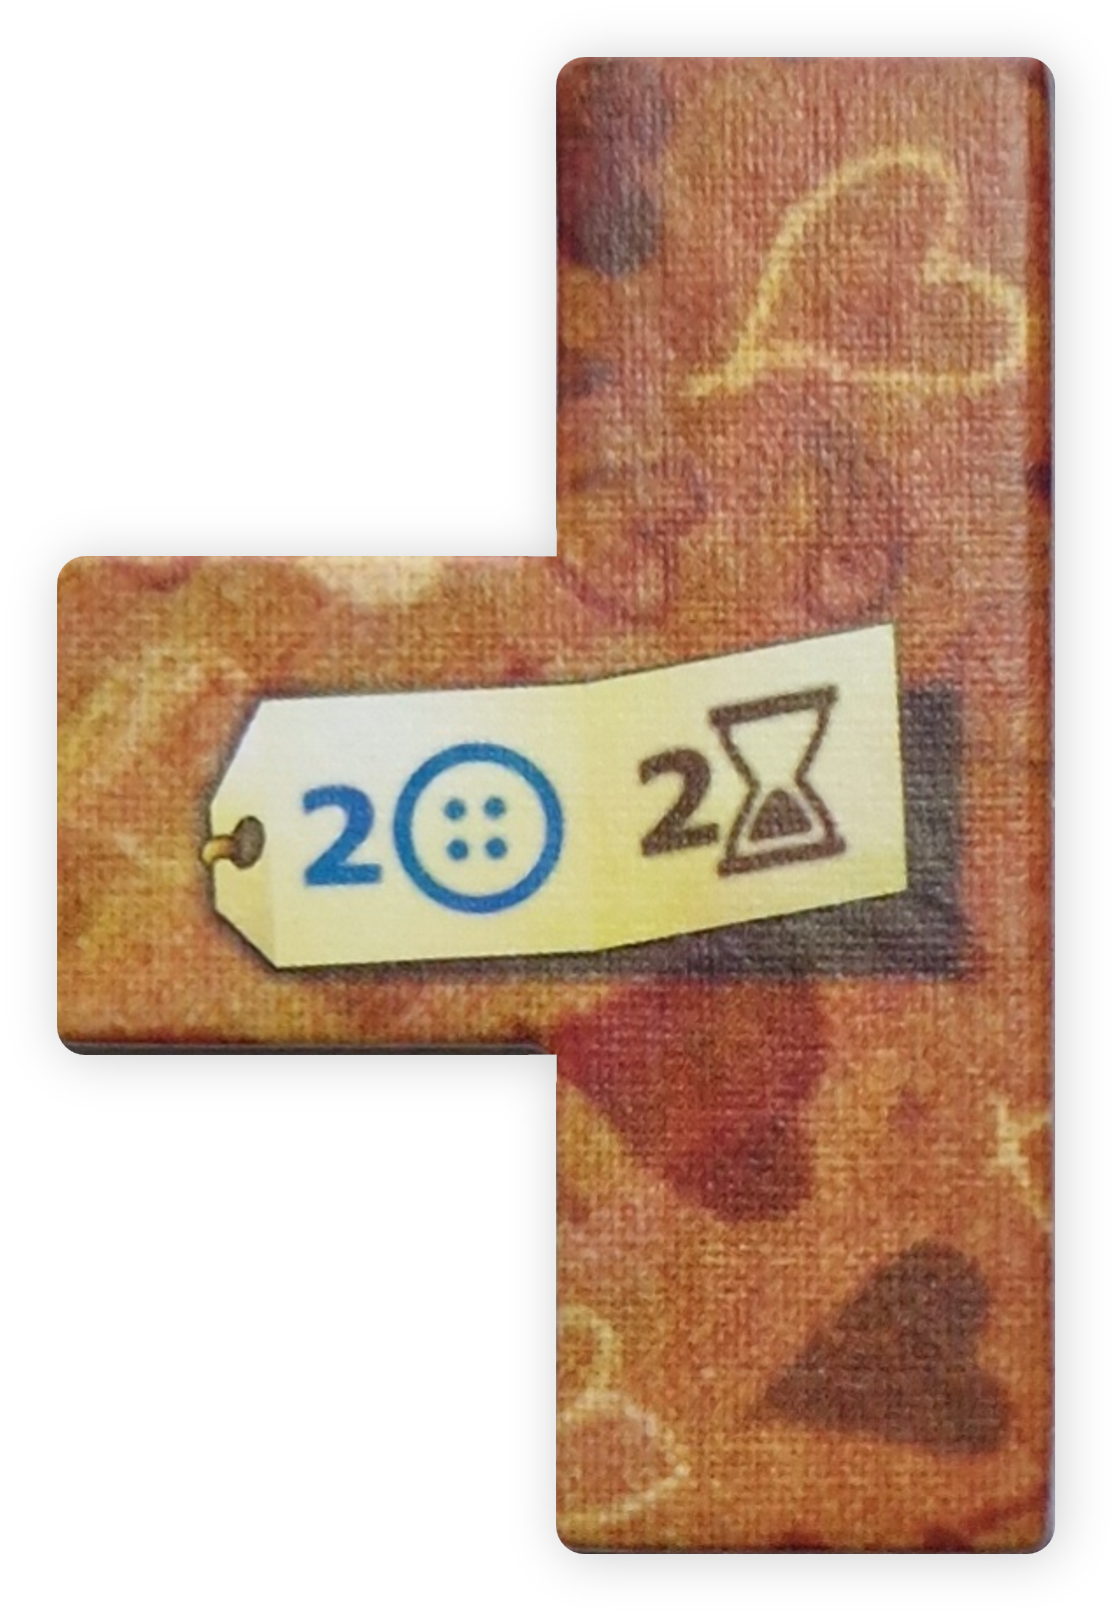
\includegraphics[width=0.2\textwidth]{res/pictures/assets/24-front.png}} & $24$ & $4$    & $2$              & $2$ & $0$ & $0$                            \\ \hline
    \adjustbox{valign=m, max width=0.2\textwidth, max height=0.1\textheight}{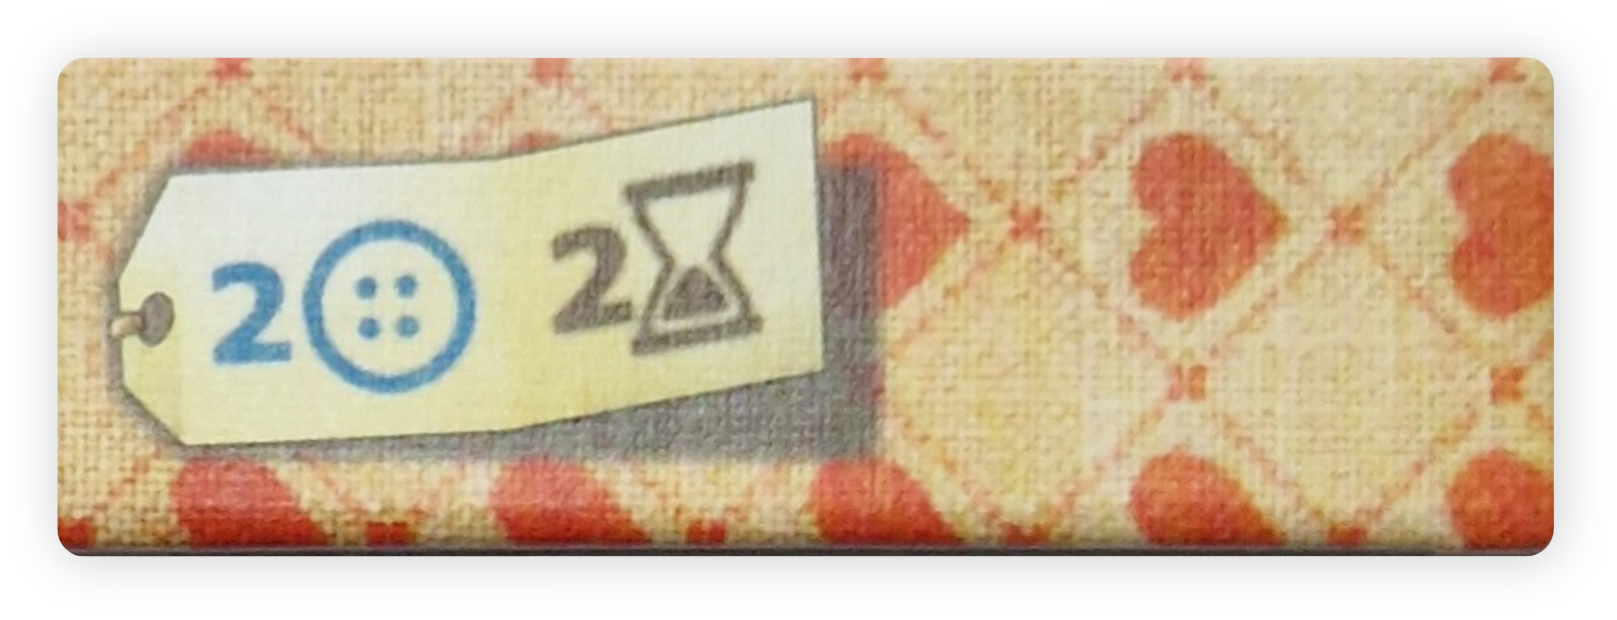
\includegraphics[width=0.2\textwidth]{res/pictures/assets/25-front.png}} & $25$ & $3$    & $2$              & $2$ & $0$ & $0$                            \\ \hline
    \adjustbox{valign=m, max width=0.2\textwidth, max height=0.1\textheight}{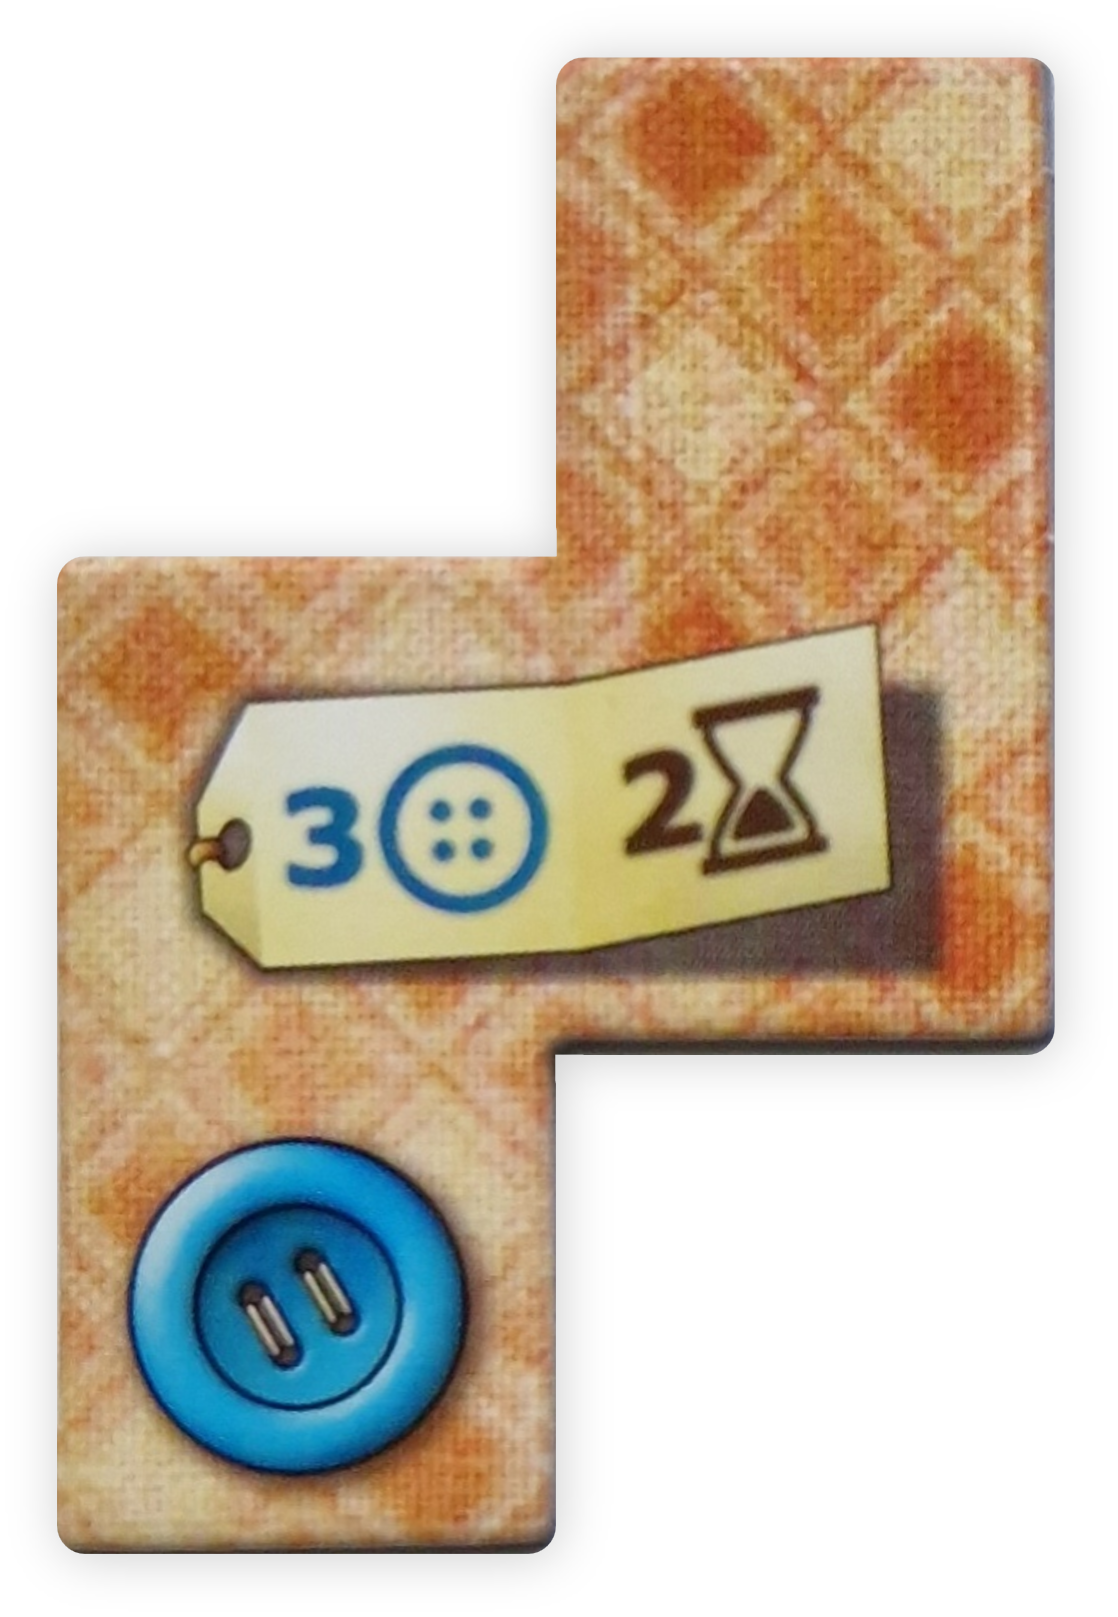
\includegraphics[width=0.2\textwidth]{res/pictures/assets/26-front.png}} & $26$ & $4$    & $3$              & $2$ & $1$ & $\frac{1}{8} = 0{,}125$        \\ \hline
    \adjustbox{valign=m, max width=0.2\textwidth, max height=0.1\textheight}{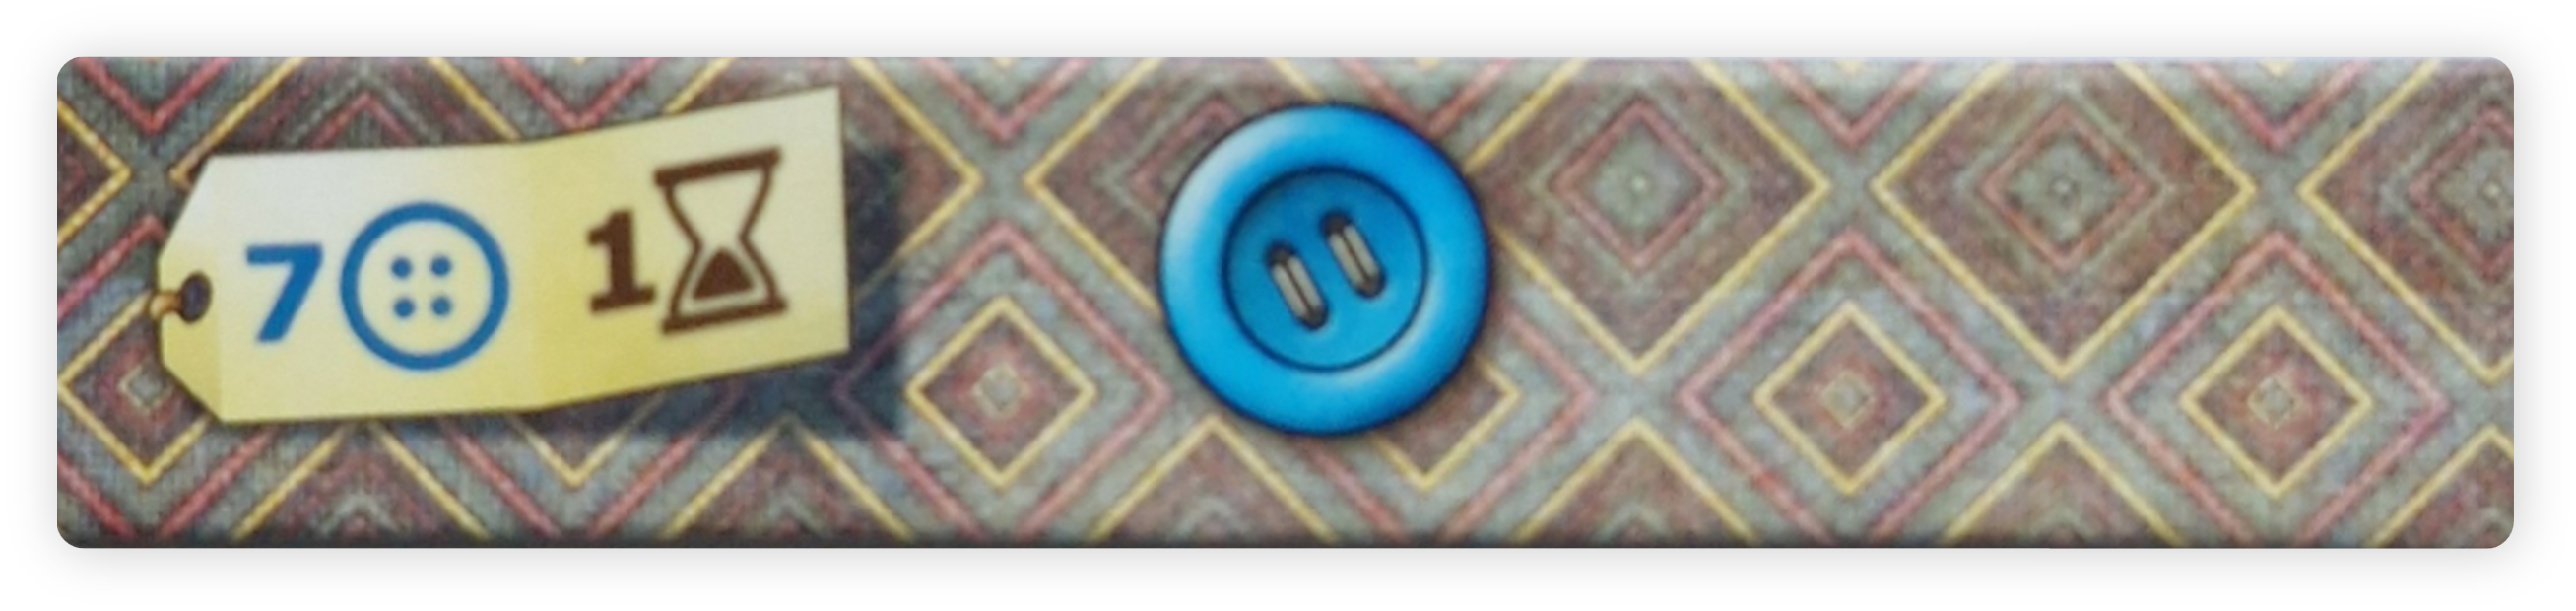
\includegraphics[width=0.2\textwidth]{res/pictures/assets/27-front.png}} & $27$ & $5$    & $7$              & $1$ & $1$ & $\frac{1}{5} = 0{,}2$          \\ \hline
    \adjustbox{valign=m, max width=0.2\textwidth, max height=0.1\textheight}{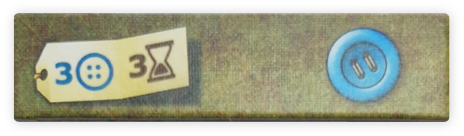
\includegraphics[width=0.2\textwidth]{res/pictures/assets/28-front.png}} & $28$ & $4$    & $3$              & $3$ & $1$ & $\frac{1}{12} \approx 0{,}083$ \\ \hline
    \adjustbox{valign=m, max width=0.2\textwidth, max height=0.1\textheight}{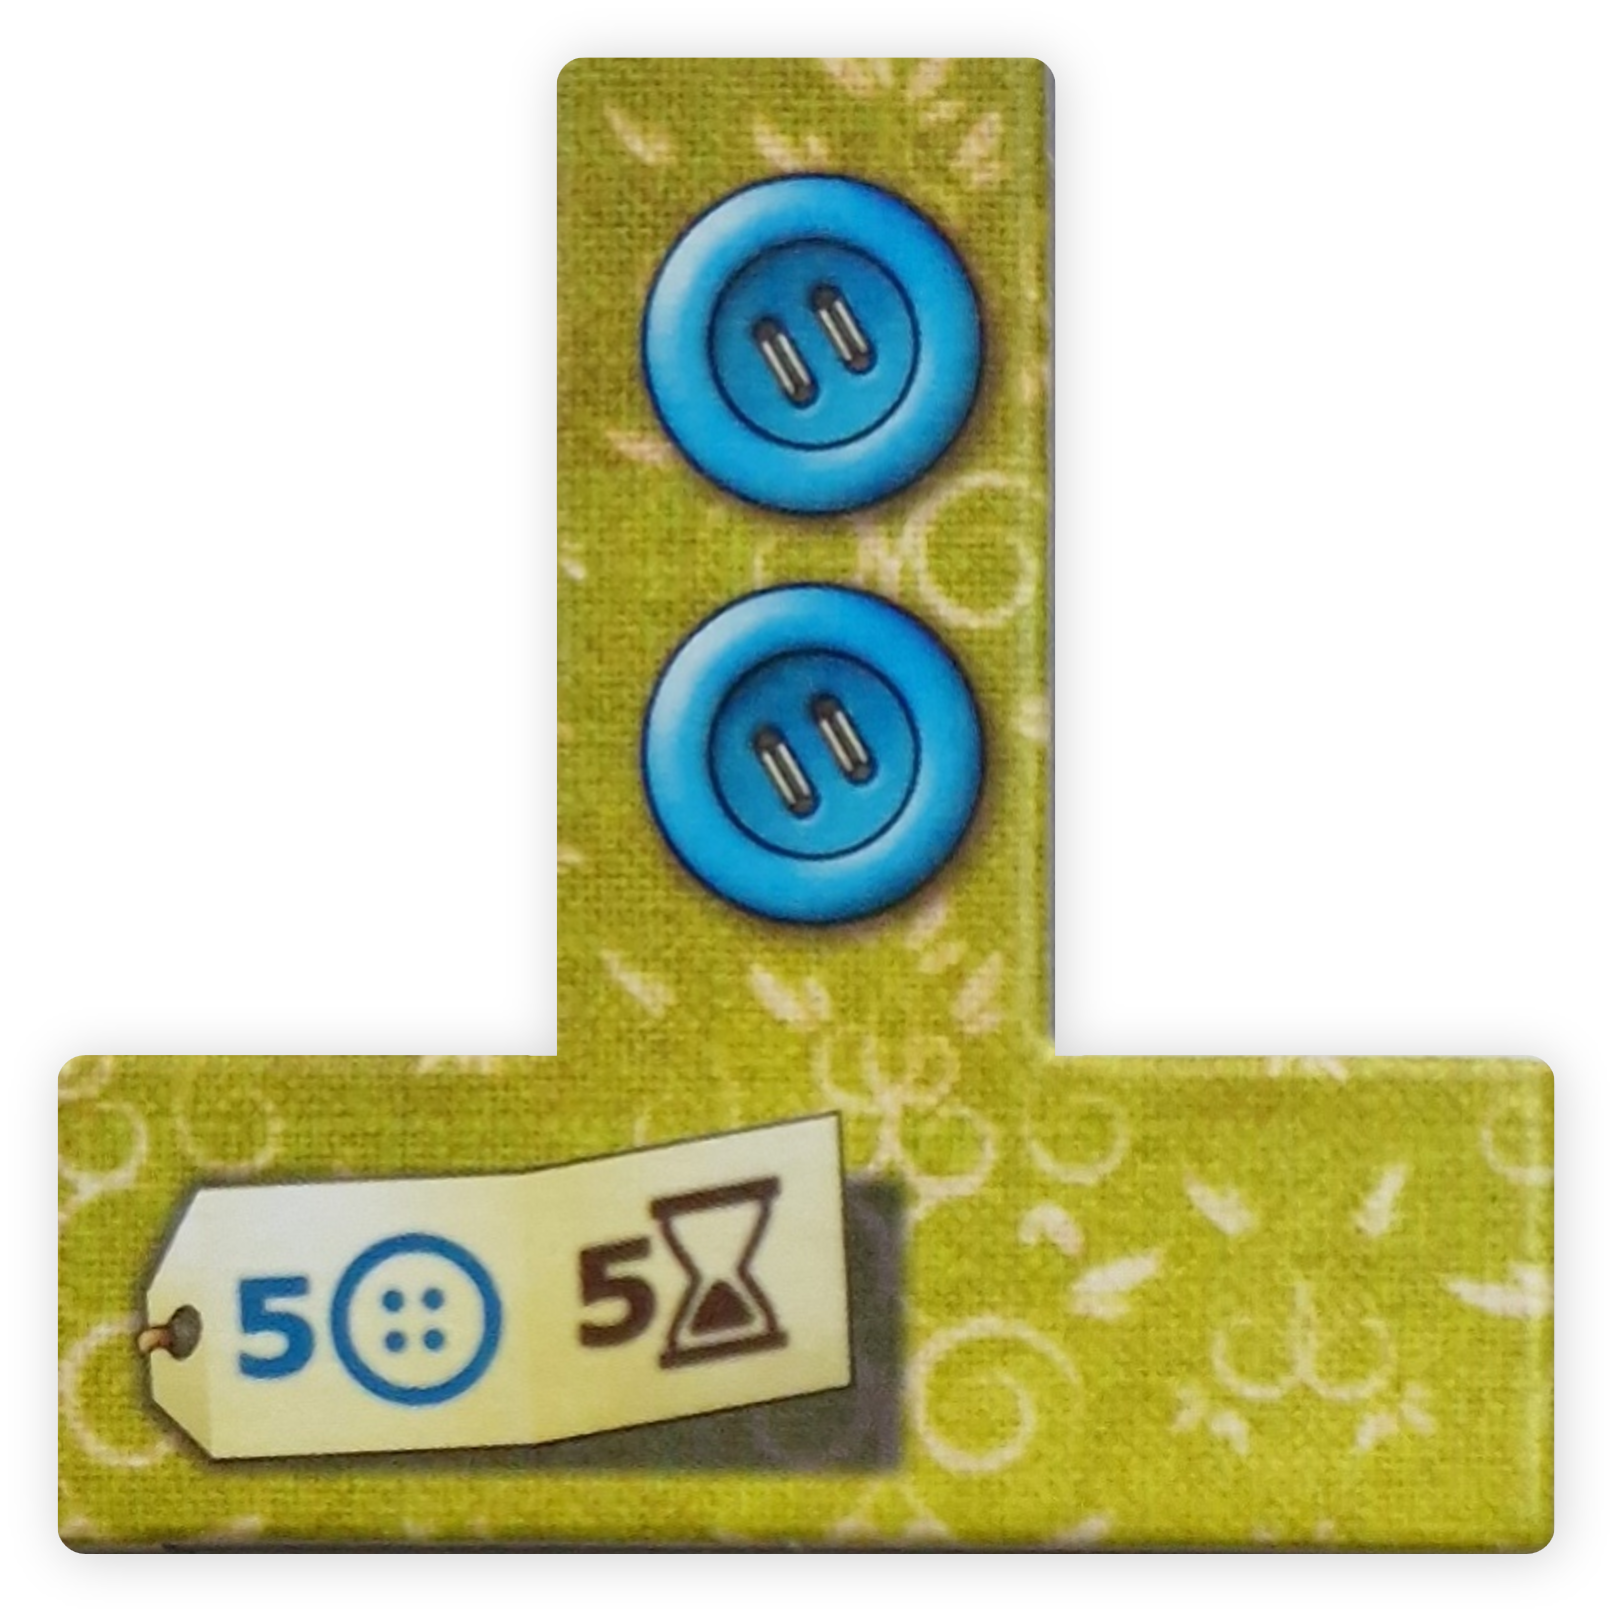
\includegraphics[width=0.2\textwidth]{res/pictures/assets/29-front.png}} & $29$ & $5$    & $5$              & $5$ & $2$ & $\frac{2}{25} = 0{,}08$        \\ \hline
    \adjustbox{valign=m, max width=0.2\textwidth, max height=0.1\textheight}{\includegraphics[width=0.2\textwidth]{res/pictures/assets/30-front.png}} & $30$ & $6$    & $3$              & $6$ & $2$ & $\frac{1}{18} \approx 0{,}056$ \\ \hline
    \adjustbox{valign=m, max width=0.2\textwidth, max height=0.1\textheight}{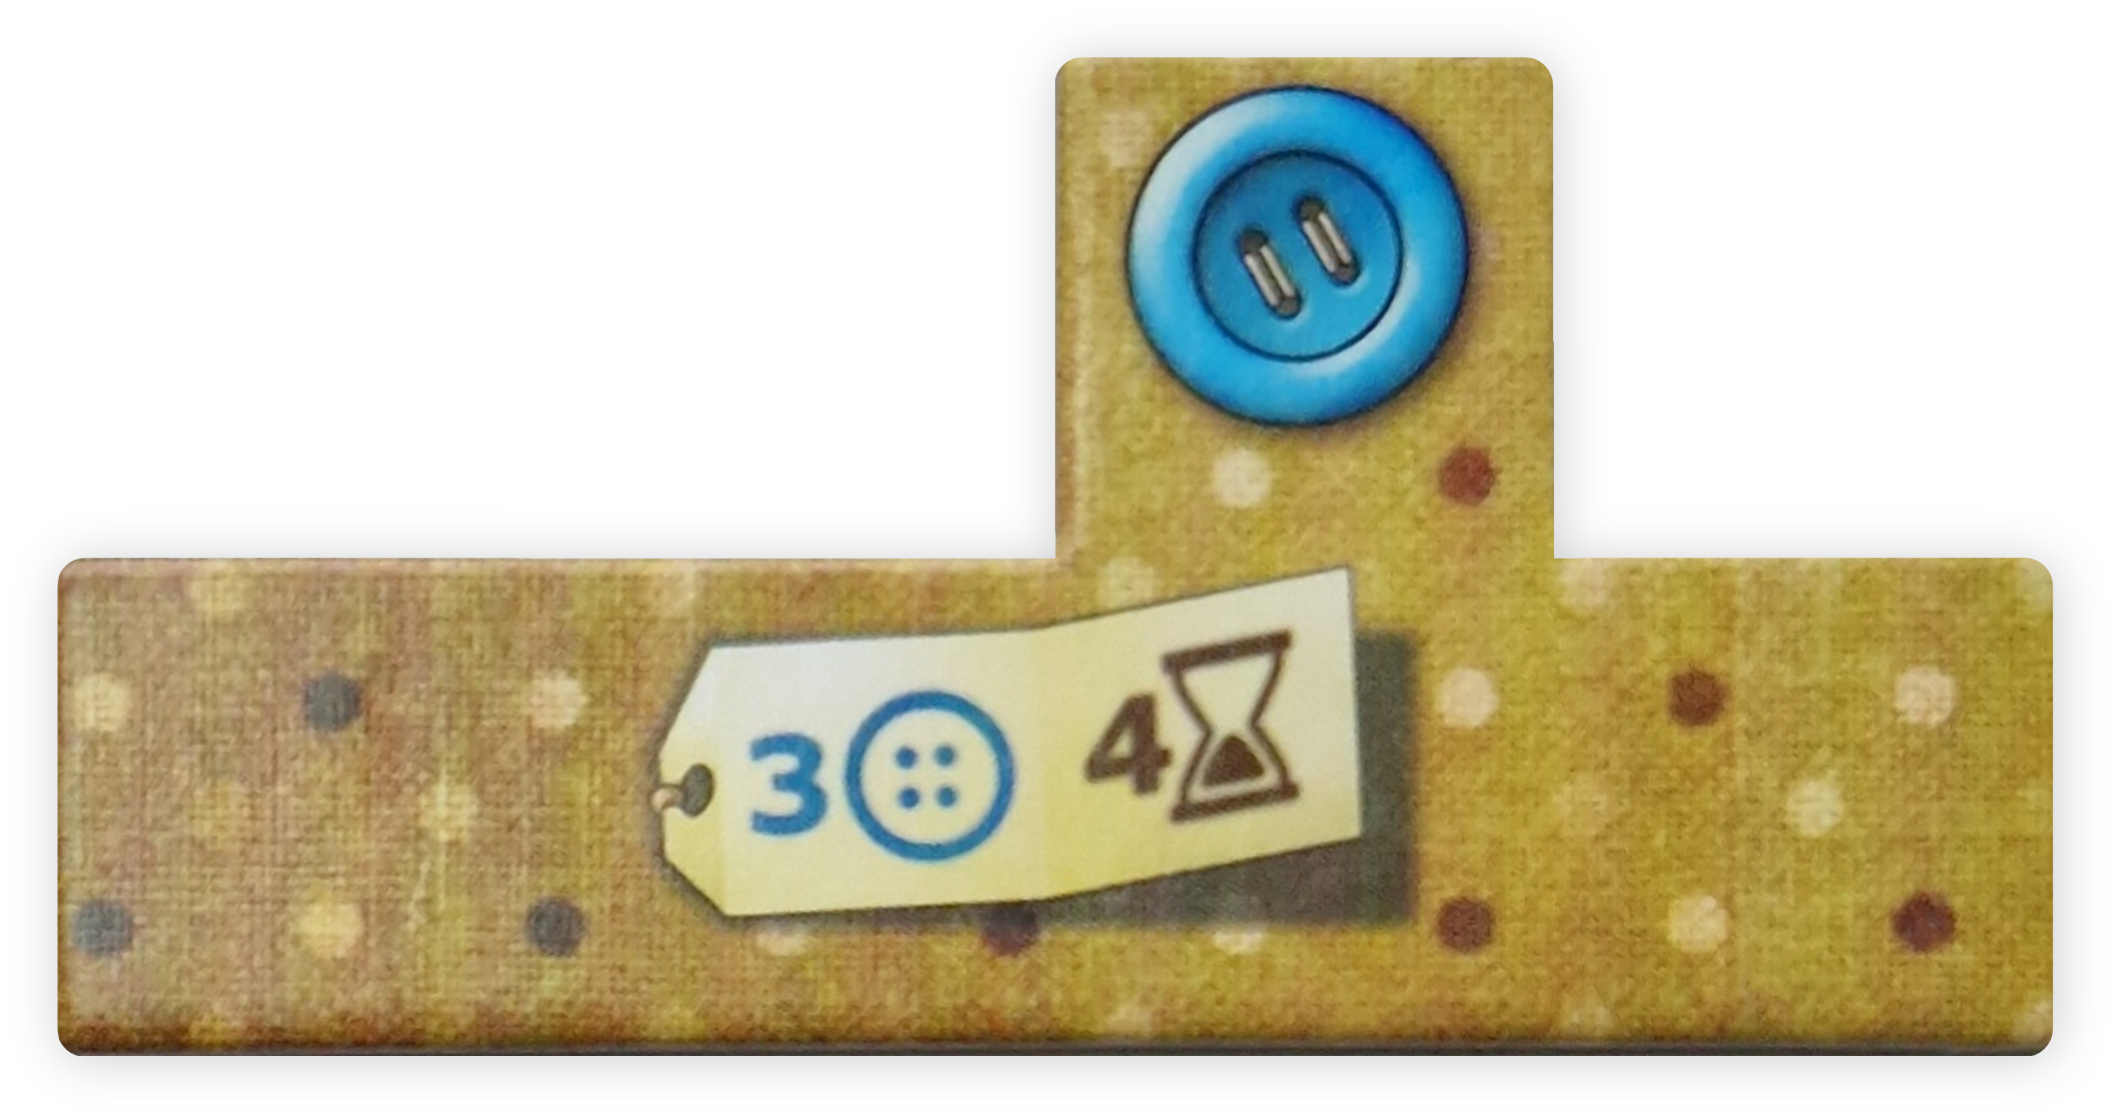
\includegraphics[width=0.2\textwidth]{res/pictures/assets/31-front.png}} & $31$ & $5$    & $3$              & $4$ & $1$ & $\frac{1}{20} = 0{,}05$        \\ \hline
    \adjustbox{valign=m, max width=0.2\textwidth, max height=0.1\textheight}{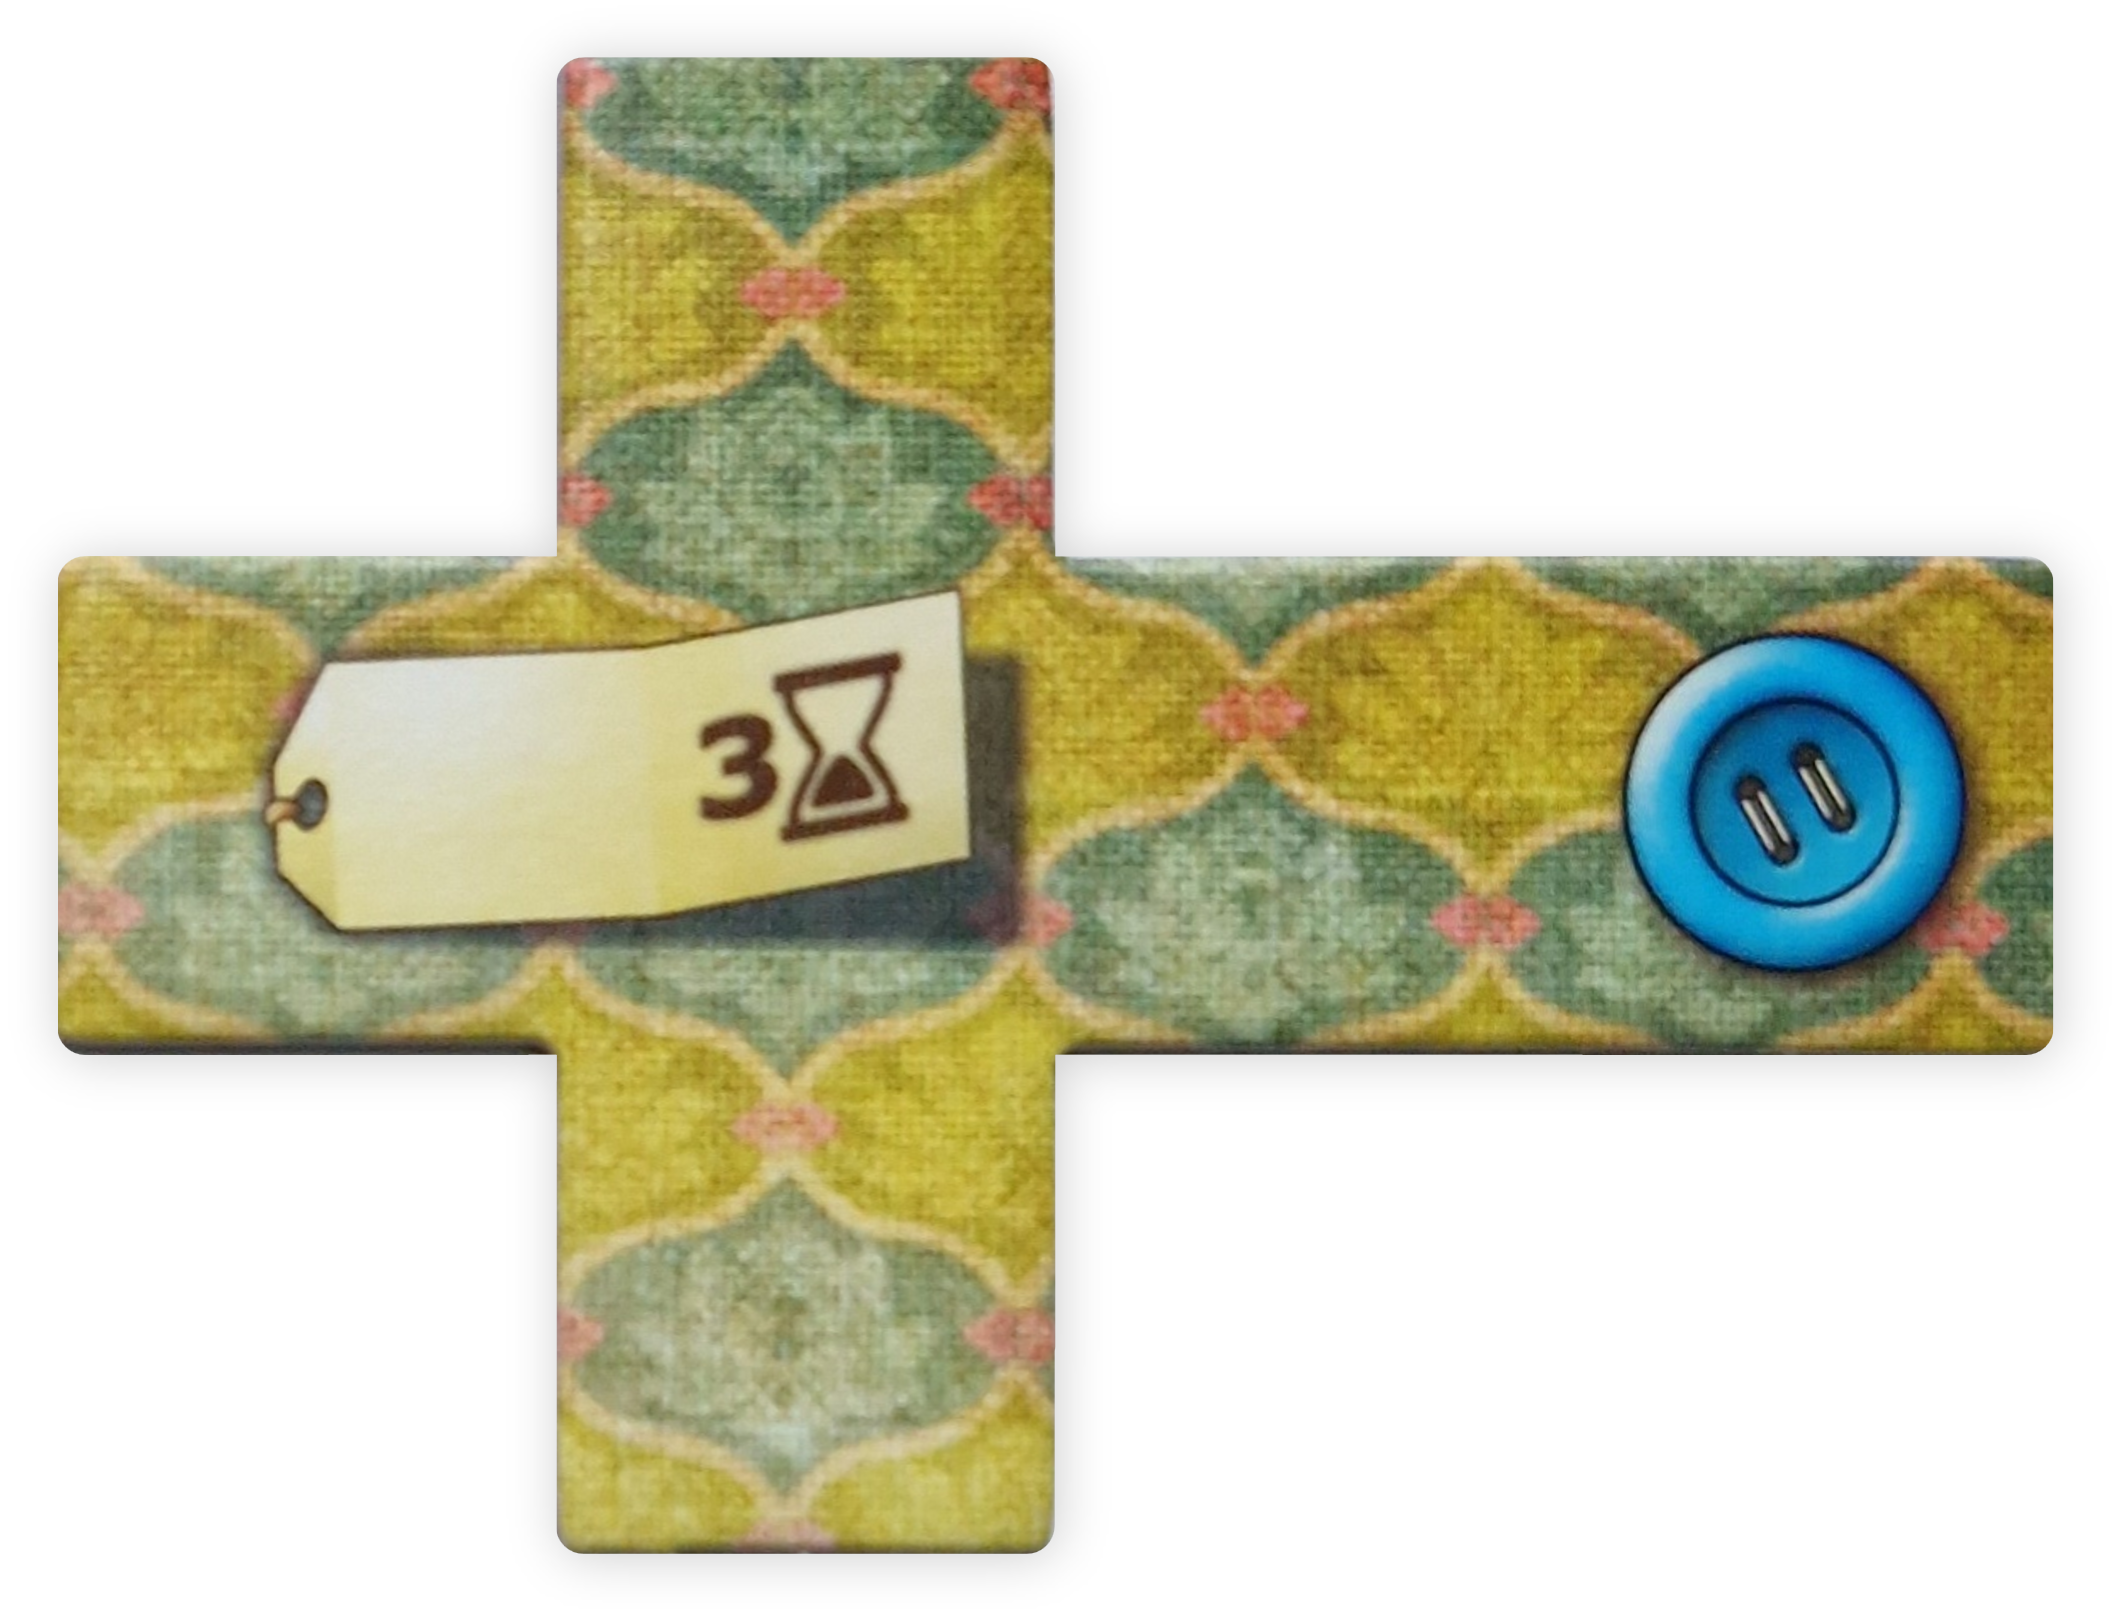
\includegraphics[width=0.2\textwidth]{res/pictures/assets/32-front.png}} & $32$ & $6$    & $0$              & $3$ & $1$ & $\frac{1}{18} \approx 0{,}056$ \\ \hline
\end{longtable}

% Reset to default
% \setlength{\tabcolsep}{6pt}